\begin{ESKDtitlePage}
  \begin{flushright}
    \textbf{ПРИЛОЖЕНИЕ Г} \enspace\enspace
  \end{flushright}
  
  \begin{center}
    % \envDiplomMinistr \\
    \envDiplomEducation \\
    \envDiplomUniversity \\
    \envDiplomCathedra \\
  \end{center}

  \vfill

  \begin{center}
    \textbf{ИНСТРУКЦИЯ ПО УСТАНОВКЕ ПО}
  \end{center}

  \vfill

  \begin{center}
    \envCode \\
  \end{center}

  \vfill

  \begin{flushright}
  \begin{minipage}[t]{.49\textwidth}
    \begin{minipage}[t]{.75\textwidth}
      \begin{flushright}
        \envDiplomTeacherInfo\\
        \hspace{0pt}\\
        \envDiplomStudentInfo\\
        \hspace{0pt}\\
        Консультанты:\\
        \envDiplomEspdInfo\\
        \hspace{0pt}\\
        \envDiplomRecendentInfo\\
      \end{flushright}
    \end{minipage}
  \end{minipage}
  \begin{minipage}[t]{.49\textwidth}
    \begin{flushright}
      \begin{minipage}[t]{.75\textwidth}
        \envDiplomTeacherInitials~\envDiplomTeacherSurname\\ % Руководитель
        \hspace{0pt}\\
        \envDiplomStudentInitials~\envDiplomStudentSurname\\ % Выполнил
        \hspace{0pt}\\
        \hspace{0pt}\\ % Консультанты:
        \envDiplomEspdInitials~\envDiplomEspdSurname\\ % по ЕСПД
        \hspace{0pt}\\
        \envDiplomRecendentInitials~\envDiplomRecendentSurname\\ % рецензент
      \end{minipage}
    \end{flushright}
  \end{minipage}
\end{flushright}


  \vfill

  \begin{center}
    \ESKDtheYear
  \end{center}
\end{ESKDtitlePage}


\newpage
\tableofcontents
\hspace{0pt}\\

% \newpage
% \ESKDstyle{title}
% \thispagestyle{plain}
% \pagestyle{plain}
% \hspace{0pt}

% \newpage
% \section{Установка редактора кода}

% \begin{enumerate}
%     \item[1.] Заходим на Github в профиль <<VSCodium>> в репозиторий <<vscodium>>.
%     \item[2.] Открываем Releases. Результат на рис.~\ref{fig:vscodium_1}.
%     \item[3.] Скачиваем установщик (Например, VSCodiumSetup-x64-*.exe).
%     \item[4.] Запускаем файл.
%     \item[5.] Соглашаемся с лицензией. Жмём <<Next>>. Результат на рис.~\ref{fig:vscodium_2}.
%     \item[6.] Выбираем папку для установки. Жмём <<Next>>. Результат на рис.~\ref{fig:vscodium_3}.
%     \item[7.] Жмём <<Next>>. Результат на рис.~\ref{fig:vscodium_4}.
%     \item[8.] Добавляем ассоциацию файлов, добавив галочку. Жмём <<Next>>. Результат на рис.~\ref{fig:vscodium_5}.
%     \item[9.] Жмём <<Install>>. Результат на рис.~\ref{fig:vscodium_6}.
% \end{enumerate}

% \begin{figure}[!phtb]
%     \centering

%     \begin{minipage}{0.49\textwidth}
%         \centering

%         \includegraphics[height=5cm]
%         {images/install/vs-codium/1.png}

%         \caption{Скриншот}

%         \label{fig:vscodium_1}
%     \end{minipage}
%     \begin{minipage}{0.49\textwidth}
%         \centering

%         \includegraphics[height=5cm]
%         {images/install/vs-codium/2.png}

%         \caption{Скриншот}

%         \label{fig:vscodium_2}
%     \end{minipage}
% \end{figure}

% \begin{figure}[!phtb]
%     \centering

%     \begin{minipage}{0.49\textwidth}
%         \centering

%         \includegraphics[height=5cm]
%         {images/install/vs-codium/3.png}

%         \caption{Скриншот}

%         \label{fig:vscodium_3}
%     \end{minipage}
%     \begin{minipage}{0.49\textwidth}
%         \centering

%         \includegraphics[height=5cm]
%         {images/install/vs-codium/4.png}

%         \caption{Скриншот}

%         \label{fig:vscodium_4}
%     \end{minipage}
% \end{figure}

% \begin{figure}[!phtb]
%     \centering

%     \begin{minipage}{0.49\textwidth}
%         \centering

%         \includegraphics[height=5cm]
%         {images/install/vs-codium/5.png}

%         \caption{Скриншот}

%         \label{fig:vscodium_5}
%     \end{minipage}
%     \begin{minipage}{0.49\textwidth}
%         \centering

%         \includegraphics[height=5cm]
%         {images/install/vs-codium/6.png}

%         \caption{Скриншот}

%         \label{fig:vscodium_6}
%     \end{minipage}
% \end{figure}

\newpage
\section{Установка NodeJS} \label{sect:nodejs}

\subsection{Установка пакетного менеджера npm и NodeJS} \label{sect:npm}

Алгоритм установки:

\begin{enumerate}
    \item[-] заходим на сайт Node JS и выбираем для скачивания LST версию (см. рисунок~\ref{fig:nodejs_1});
    \item[-] жмём <<Next>>. (см. рисунок~\ref{fig:nodejs_2});
    \item[-] cоглашаемся с лицензией и жмём <<Next>> (см. рисунок~\ref{fig:nodejs_3});
    \item[-] выбираем папку для установки и жмём <<Next>> (см. рисунок~\ref{fig:nodejs_4});
    \item[-] жмём <<Next>> (см. рисунок~\ref{fig:nodejs_5});
    \item[-] жмём <<Next>> (см. рисунок~\ref{fig:nodejs_6});
    \item[-] жмём <<Install>> (см. рисунок~\ref{fig:nodejs_7});
    \item[-] жмём <<Finish>> (см. рисунок~\ref{fig:nodejs_8});
    \item[-] для проверки корректности установки открываем командную строку <<Win>> + <<R>>, <<cmd>>, <<Enter>>;
    \item[-] вводим команду <<node -v>>, а если нет ошибки, то есть вывелась версия, например, <<v18.16.0>>, то NodeJS установлен;
    \item[-] вводим команду <<npm -v>>, а если нет ошибки, то есть вывелась версия, например, <<9.5.1>>, то пакетный менеджер npm установлен.
\end{enumerate}

\subsection{Установка пакетного менеджера yarn}

Алгоритм установки:
\begin{enumerate}
    \item[-] открываем командную строку <<Win>> + <<R>>, <<cmd>>, <<Enter>>;
    \item[-] вводим команду <<npm i -g yarn>>;
    \item[-] вводим команду <<yarn -v>>, а если нет ошибки, то есть вывелась версия, например, <<1.22.19>>, то пакетный менеджер yarn установлен.
\end{enumerate}

\begin{figure}[!phtb]
    \centering

    \begin{minipage}{0.49\textwidth}
        \centering

        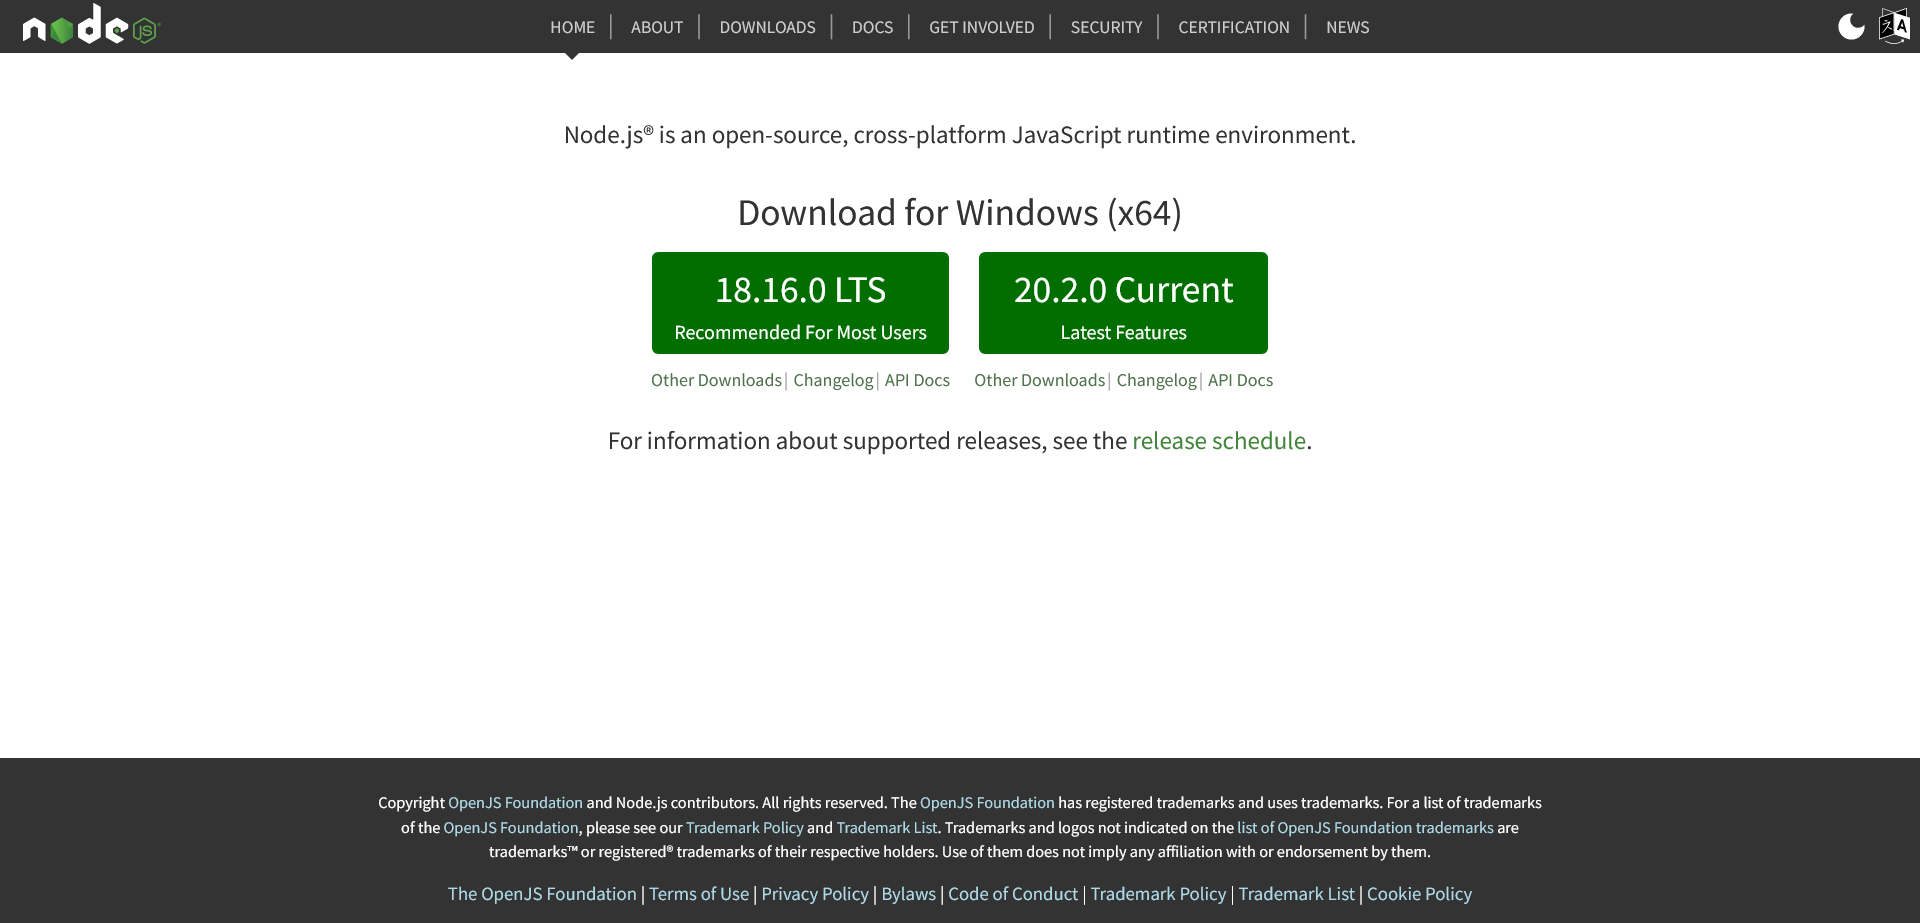
\includegraphics[height=4cm]
        {images/install/node-js/1.png}

        \caption{Скриншот}

        \label{fig:nodejs_1}
    \end{minipage}
    \begin{minipage}{0.49\textwidth}
        \centering

        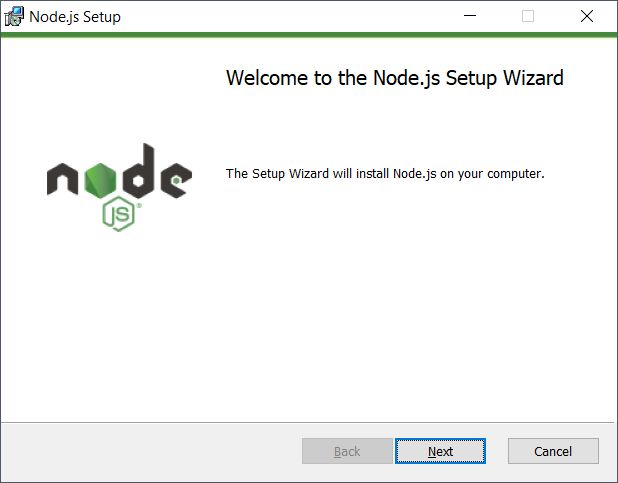
\includegraphics[height=4cm]
        {images/install/node-js/2.png}

        \caption{Скриншот}

        \label{fig:nodejs_2}
    \end{minipage}
\end{figure}

\begin{figure}[!phtb]
    \centering

    \begin{minipage}{0.49\textwidth}
        \centering

        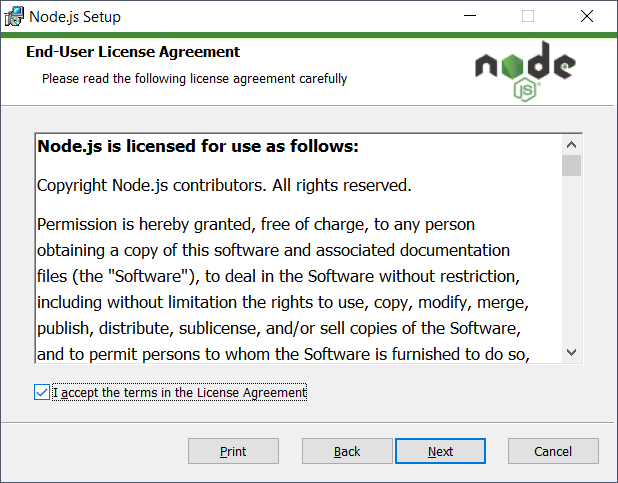
\includegraphics[height=5cm]
        {images/install/node-js/3.png}

        \caption{Скриншот}

        \label{fig:nodejs_3}
    \end{minipage}
    \begin{minipage}{0.49\textwidth}
        \centering

        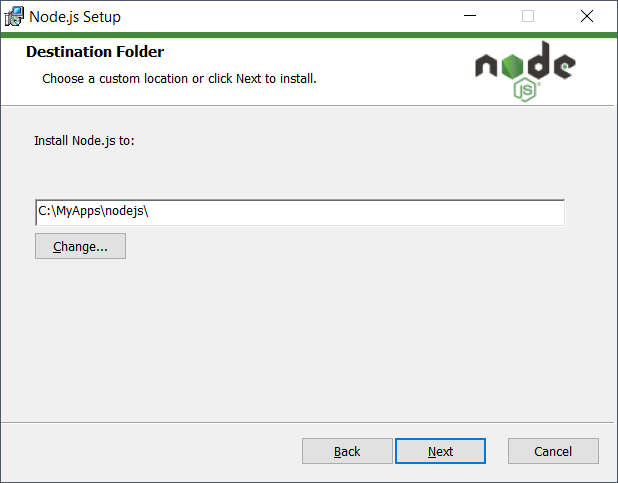
\includegraphics[height=5cm]
        {images/install/node-js/4.png}

        \caption{Скриншот}

        \label{fig:nodejs_4}
    \end{minipage}
\end{figure}

\begin{figure}[!phtb]
    \centering

    \begin{minipage}{0.49\textwidth}
        \centering

        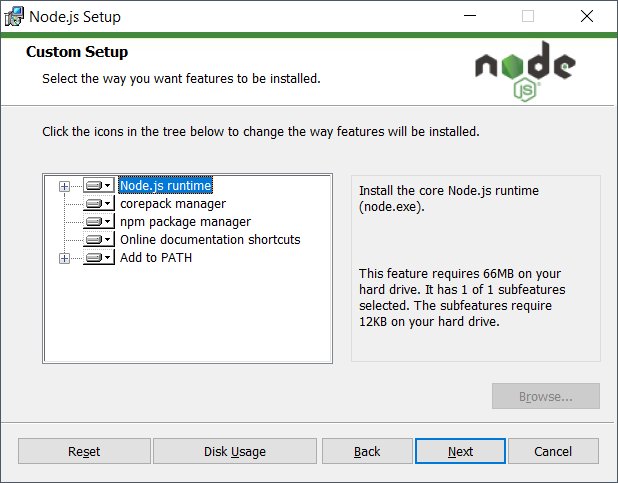
\includegraphics[height=5cm]
        {images/install/node-js/5.png}

        \caption{Скриншот}

        \label{fig:nodejs_5}
    \end{minipage}
    \begin{minipage}{0.49\textwidth}
        \centering

        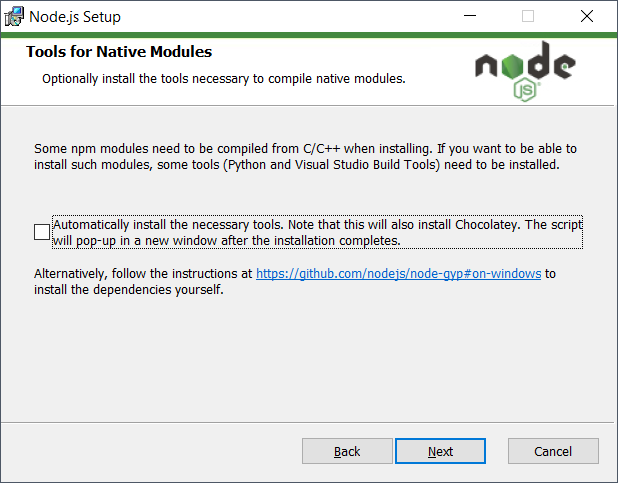
\includegraphics[height=5cm]
        {images/install/node-js/6.png}

        \caption{Скриншот}

        \label{fig:nodejs_6}
    \end{minipage}
\end{figure}

\begin{figure}[!phtb]
    \centering

    \begin{minipage}{0.49\textwidth}
        \centering

        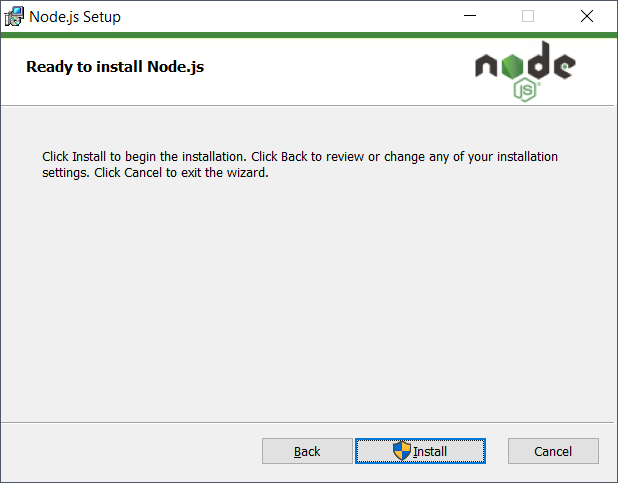
\includegraphics[height=5cm]
        {images/install/node-js/7.png}

        \caption{Скриншот}

        \label{fig:nodejs_7}
    \end{minipage}
    \begin{minipage}{0.49\textwidth}
        \centering

        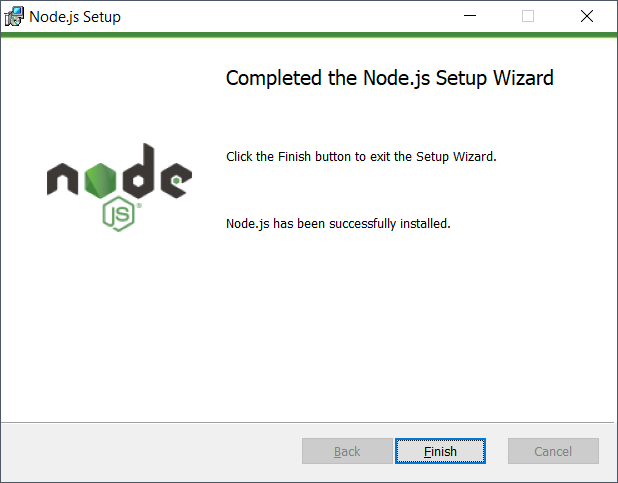
\includegraphics[height=5cm]
        {images/install/node-js/8.png}

        \caption{Скриншот}

        \label{fig:nodejs_8}
    \end{minipage}
\end{figure}

\newpage
\section{Установка Docker и Docker-compose} \label{sect:docker}

Алгоритм установки:
\begin{enumerate}
    \item[-] заходим на сайт Docker и скачиваем установщик. Результат на рис.~\ref{fig:docker_1}.
    \item[-] запускаем установщик;
    \item[-] убираем галочку создания ярлыка на рабочем столе по желанию (при каждом запуске компьютера нужно будет запускать Docker снова);
    \item[-] жмём <<OK>> (см. рисунок~\ref{fig:docker_2});
    \item[-] ждём установки (см. рисунок~\ref{fig:docker_3});
    \item[-] жмём <<Close and restart>> (см. рисунок~\ref{fig:docker_4});
    \item[-] после перезапуска компьютера запускаем Docker;
    \item[-] жмём <<Accept>> (см. рисунок~\ref{fig:docker_5});
    \item[-] появилась предупреждение, что Docker работает с WSLv2 (Windows Subsystem Linux version 2), а у нас WSLv1 (Windows Subsystem Linux version 1) (см. рисунок~\ref{fig:docker_6});
    \item[-] переходим по этой ссылке;
    \item[-] на сайте ищем ссылку для скачивания установщика (см. рисунок~\ref{fig:docker_7});
    \item[-] запускаем установщик;
    \item[-] жмём <<Next>> (см. рисунок~\ref{fig:docker_8});
    \item[-] жмём <<Finish>> (см. рисунок~\ref{fig:docker_9});
    \item[-] перезапускаем компьютер;
    \item[-] открываем Docker (см. рисунок~\ref{fig:docker_10});
    \item[-] для проверки корректности установки открываем командную строку <<Win>> + <<R>>, <<cmd>>, <<Enter>>;
    \item[-] вводим команду <<docker -v>>, а если нет ошибки, то есть вывелась версия, например, <<Docker version 23.0.5>>, то Docker установлен;
    \item[-] вводим команду <<docker-compose -v>>, а если нет ошибки, то есть вывелась версия, например, <<Docker-compose version 2.17.3>>, то docker-compose установлен.
\end{enumerate}

\begin{figure}[!phtb]
    \centering

    \begin{minipage}{0.49\textwidth}
        \centering

        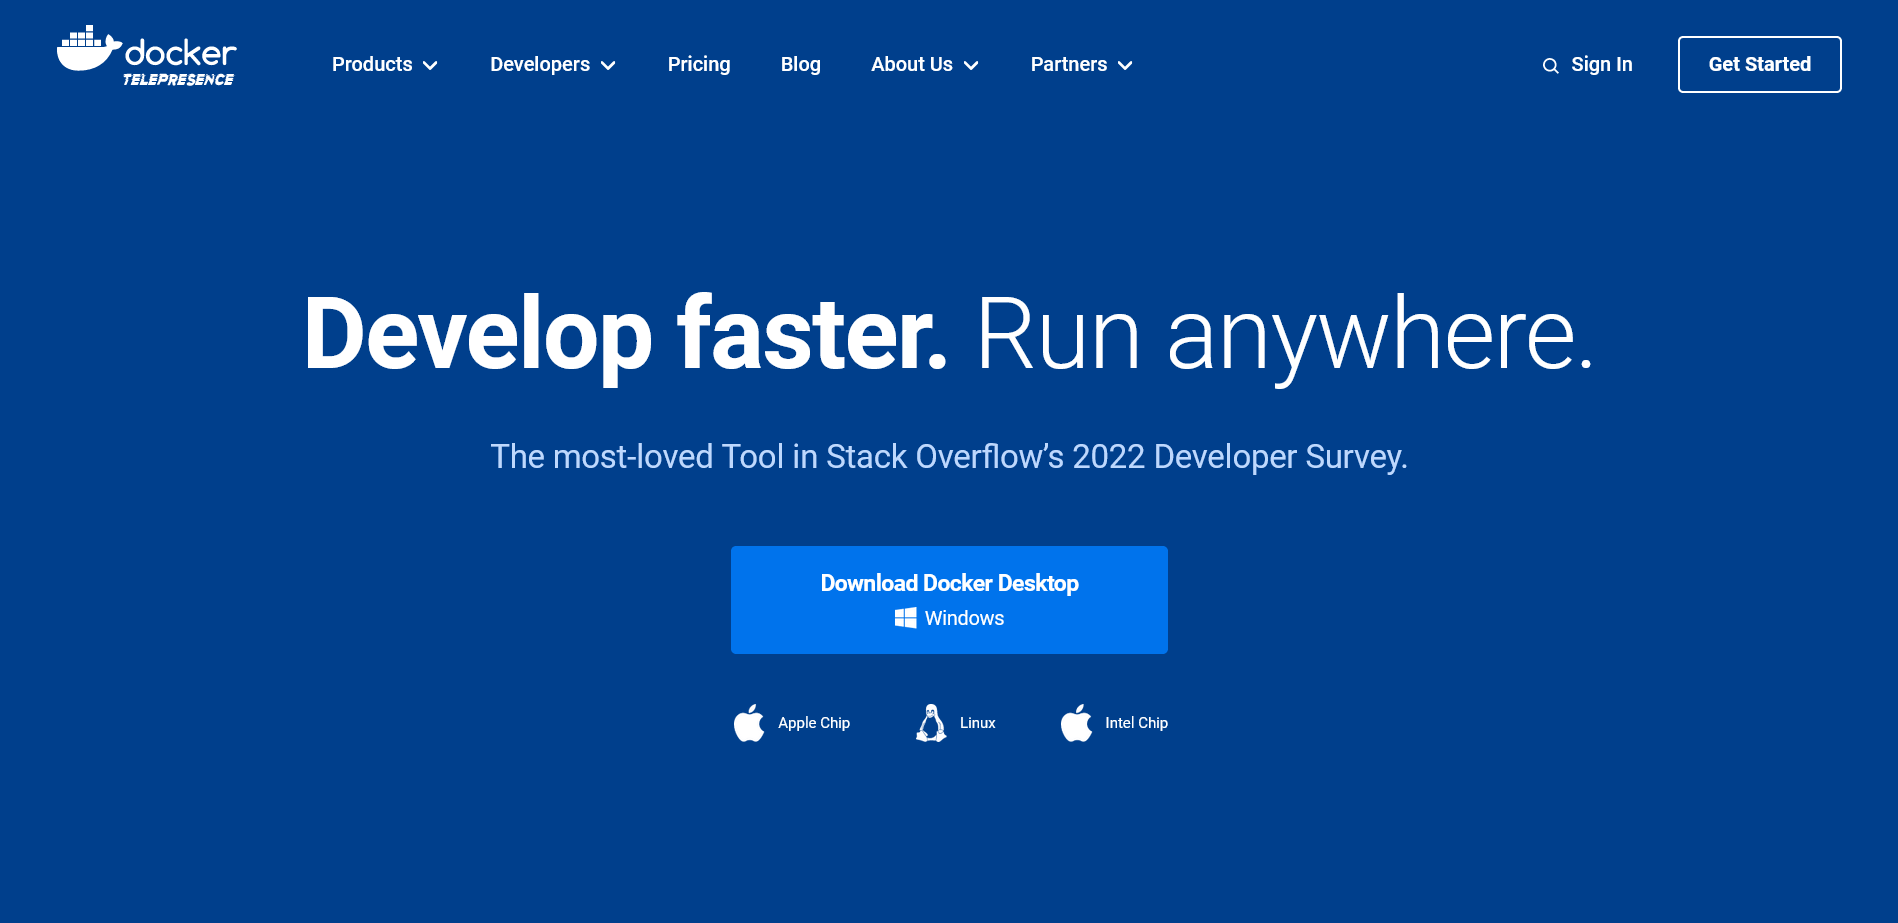
\includegraphics[width=0.99\textwidth]
        {images/install/docker/1.png}

        \caption{Скриншот}

        \label{fig:docker_1}
    \end{minipage}
    \begin{minipage}{0.49\textwidth}
        \centering

        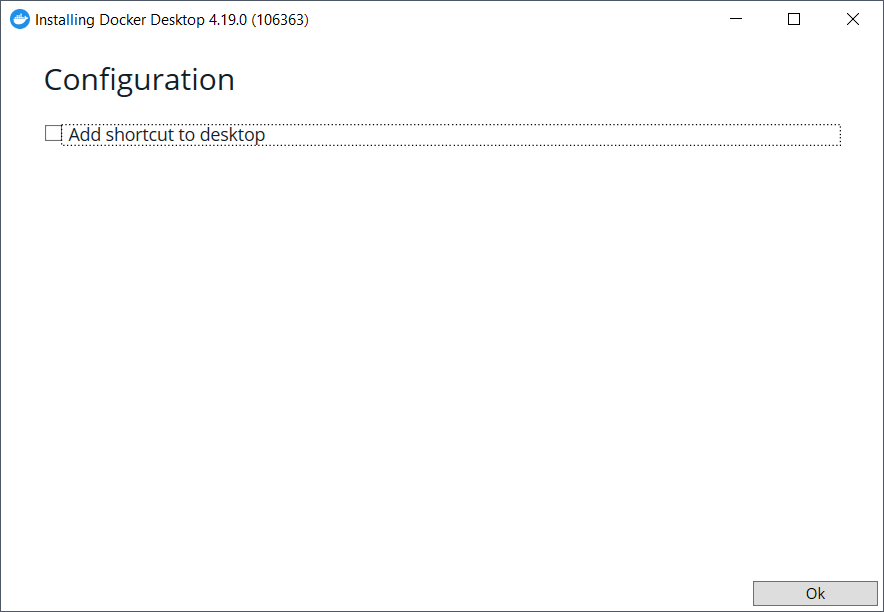
\includegraphics[width=0.99\textwidth]
        {images/install/docker/2.png}

        \caption{Скриншот}

        \label{fig:docker_2}
    \end{minipage}
\end{figure}

\begin{figure}[!phtb]
    \centering

    \begin{minipage}{0.49\textwidth}
        \centering

        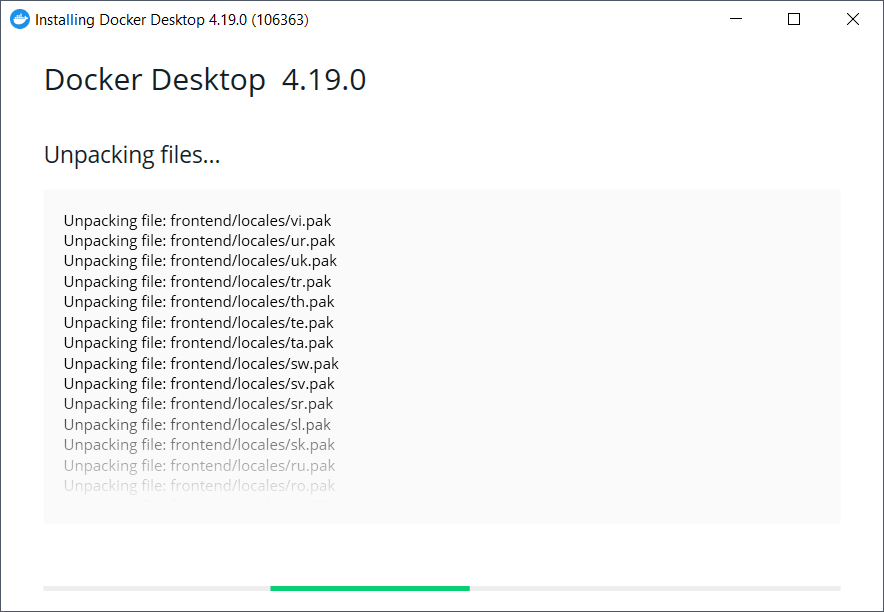
\includegraphics[width=0.99\textwidth]
        {images/install/docker/3.png}

        \caption{Скриншот}

        \label{fig:docker_3}
    \end{minipage}
    \begin{minipage}{0.49\textwidth}
        \centering

        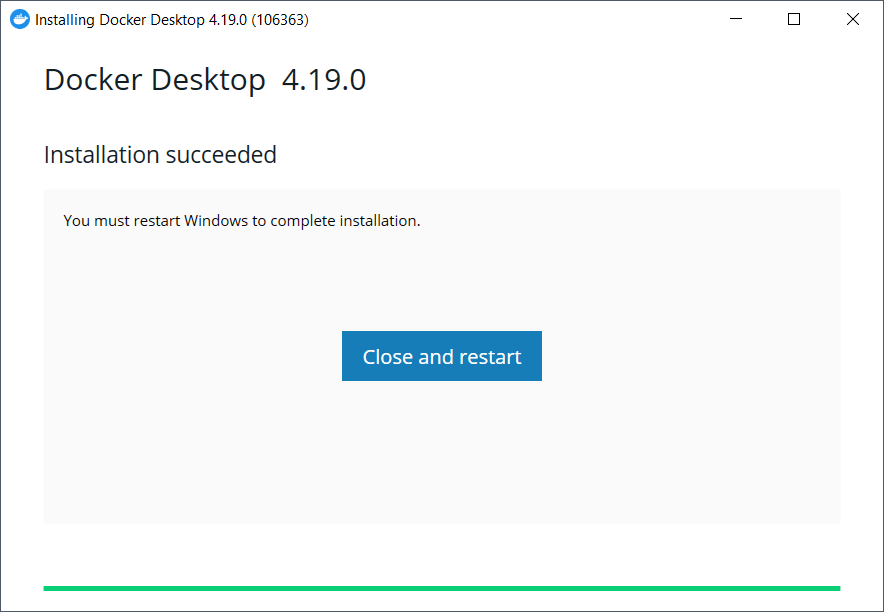
\includegraphics[width=0.99\textwidth]
        {images/install/docker/4.png}

        \caption{Скриншот}

        \label{fig:docker_4}
    \end{minipage}
\end{figure}

\begin{figure}[!phtb]
    \centering

    \begin{minipage}{0.49\textwidth}
        \centering

        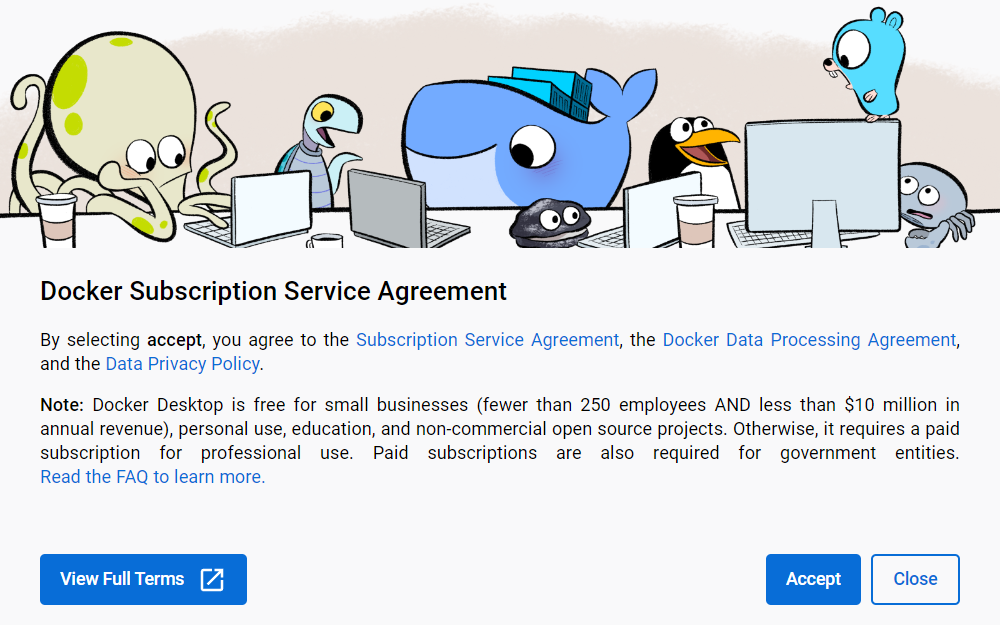
\includegraphics[width=0.99\textwidth]
        {images/install/docker/5.png}

        \caption{Скриншот}

        \label{fig:docker_5}
    \end{minipage}
    \begin{minipage}{0.49\textwidth}
        \centering

        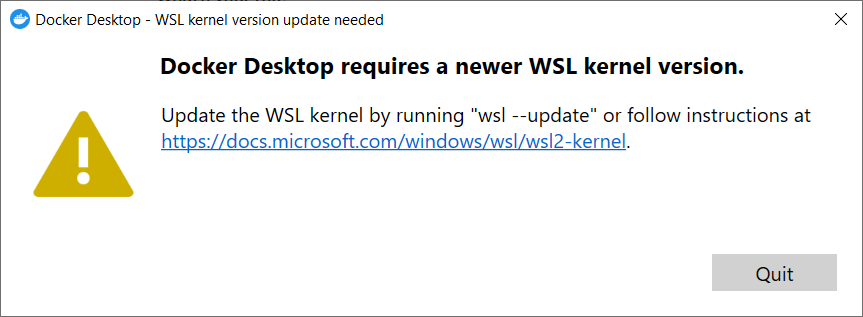
\includegraphics[width=0.99\textwidth]
        {images/install/docker/6.png}

        \caption{Скриншот}

        \label{fig:docker_6}
    \end{minipage}
\end{figure}

\begin{figure}[!phtb]

    \centering

    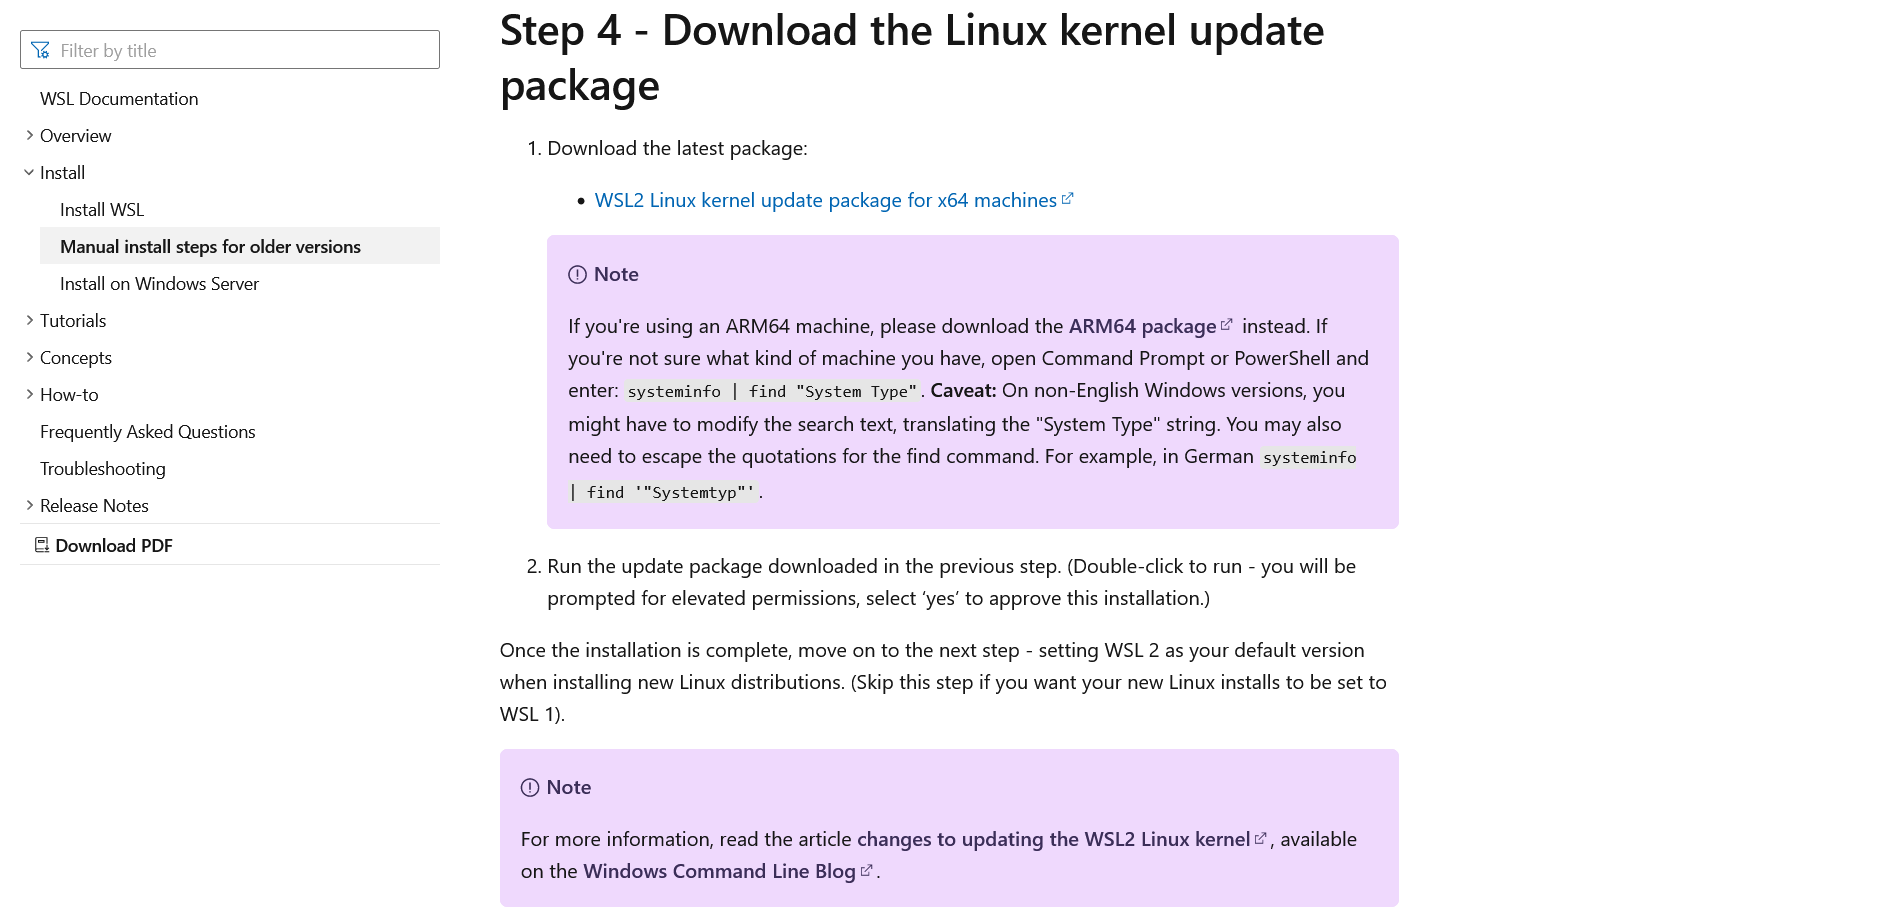
\includegraphics[height=8cm]
    {images/install/docker/7.png}

    \caption{Скриншот}

    \label{fig:docker_7}

\end{figure}

\begin{figure}[!phtb]
    \centering

    \begin{minipage}{0.49\textwidth}
        \centering

        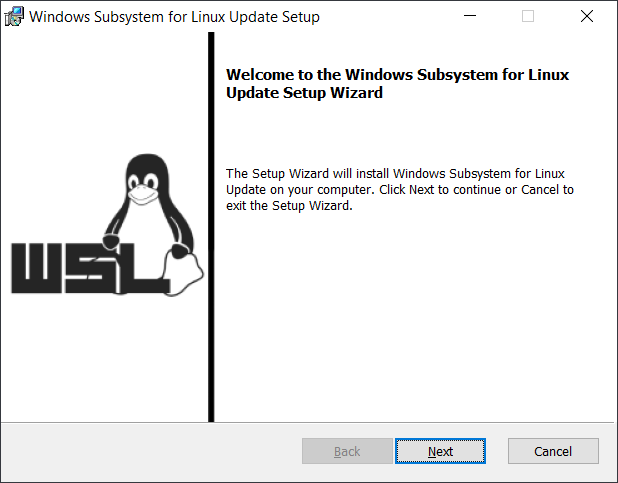
\includegraphics[width=0.99\textwidth]
        {images/install/docker/8.png}

        \caption{Скриншот}

        \label{fig:docker_8}
    \end{minipage}
    \begin{minipage}{0.49\textwidth}
        \centering

        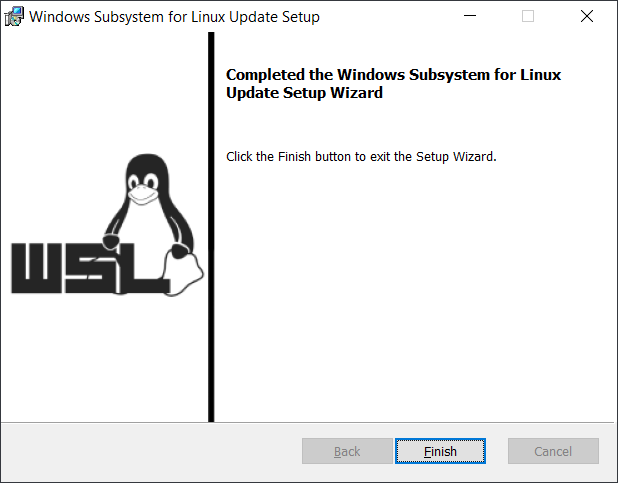
\includegraphics[width=0.99\textwidth]
        {images/install/docker/9.png}

        \caption{Скриншот}

        \label{fig:docker_9}
    \end{minipage}
\end{figure}

\begin{figure}[!phtb]

    \centering

    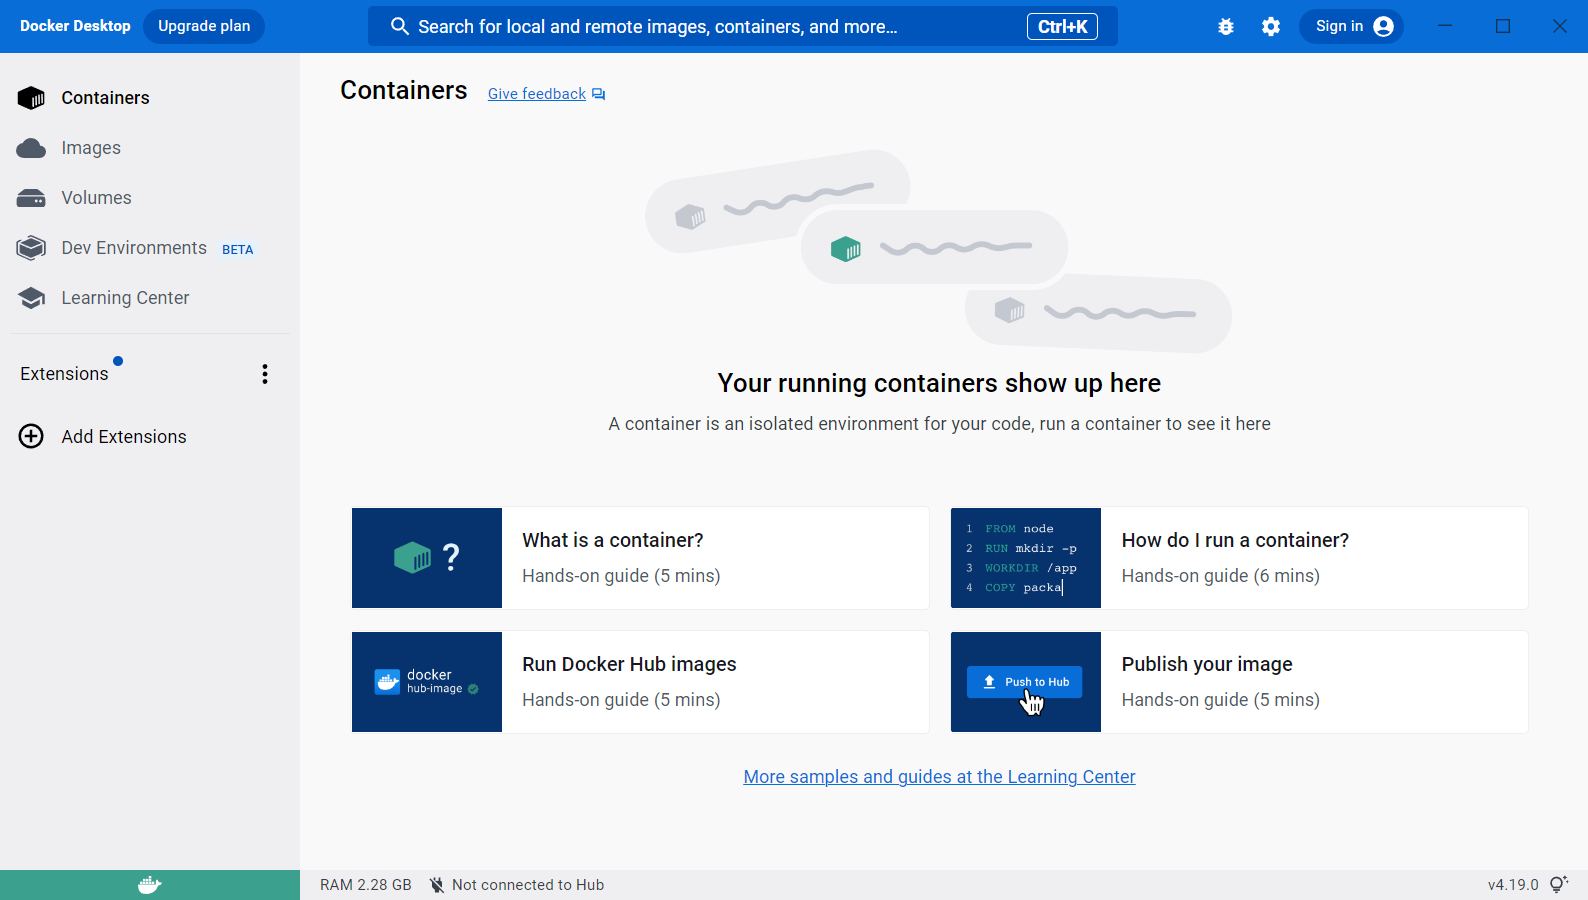
\includegraphics[height=6cm]
    {images/install/docker/10.png}

    \caption{Скриншот}

    \label{fig:docker_10}

\end{figure}

\newpage
\section{Запуск серверной части для разработки} \label{sect:backend}

\subsection{Запуск MySQL в Docker-контейнере}

Перед запуском необходимо иметь установленный Docker и docker-compose (см. главу~\ref{sect:docker}).

Алгоритм запуска MySQL в Docker-контейнере:
\begin{enumerate}
    \item[-] копируем с диска папку <<dp\_backend>> себе на компьютер;
    \item[-] открываем консоль;
    \item[-] вводим команду <<cd docker>>;
    \item[-] вводим команду <<cd db>>;
    \item[-] вводим команду <<cd dev-mysql>>;
    \item[-] если нет файла <<.env>>, то создаем этот файл на основе <<.env.example>>;
    \item[-] запускаем контейнер командой <<docker-compose up>>;
    \item[-] открываем http://localhost:11112 (если нужен phpmyadmin).
\end{enumerate}

\subsection{Запуск миграций}

Перед запуском миграций, должна быть запущена БД, и занесены данные в файл <<.env>>,
также должна быть установлена NodeJS (см. главу~\ref{sect:nodejs}).

Алгоритм запуска миграций:
\begin{enumerate}
    \item[-] открываем папку <<dp\_backend>>;
    \item[-] открываем консоль;
    \item[-] переходим папку sources командой: <<cd sources>>;
    \item[-] если не установлены npm пакеты, то есть нет папки node\_modules, то устанавливаем командой <<yarn>>;
    \item[-] если не создан файл <<dev.env>>, то создаем на основе файла\\ <<dev.env.example>>;
    \item[-] запускаем миграции командой <<yarn dev-migr-run>>.
\end{enumerate}

Откат одной миграции производится командой <<yarn dev-migr-rev>>.

Командой <<yarn dev-migr-gen src/migrations/наименование>> производится создание миграции.

\subsection{Запуск для разработки серверной части}

Перед запуском серверной части должна быть установлена NodeJS (см. главу~\ref{sect:nodejs}).

Алгоритм запуска серверной части:
\begin{enumerate}
    \item[-] открываем папку <<dp\_backend>>;
    \item[-] открываем консоль;
    \item[-] переходим папку sources командой: <<cd sources>>.
    \item[-] если не установлены пакеты npm, то есть нет папки node\_modules, то устанавливаем командой <<yarn>>;
    \item[-] если не создан файл <<dev.env>>, то создаем на основе файла\\ <<dev.env.example>>;
    \item[-] запускаем серверную часть командой <<yarn dev-start>>;
    \item[-] открываем http://localhost:11111/api/v1.
\end{enumerate}

\newpage
\section{Запуск панели администратора для разработки}

Перед запуском панели администратора должна быть установлена NodeJS (см. главу~\ref{sect:nodejs}).

Панель администратора не будет работать без запущеной серверной части (см. главу~\ref{sect:backend}).

Алгоритм запуска серверной части:
\begin{enumerate}
    \item[-] открываем папку <<dp\_admin\_panel>>;
    \item[-] открываем консоль;
    \item[-] переходим папку sources командой: <<cd sources>>.
    \item[-] если не установлены пакеты npm, то есть нет папки node\_modules, то устанавливаем командой <<yarn>>;
    \item[-] если не создан файл <<.env>>, то создаем на основе файла <<.env.example>>;
    \item[-] запускаем командой <<yarn start>>;
    \item[-] открываем http://localhost:3000.
\end{enumerate}

Для смены порта в файле прописать <<PORT=3001>>.

\newpage
\section{Запуск панели менеджера для разработки}

Перед запуском панели менеджера должна быть установлена NodeJS (см. главу~\ref{sect:nodejs}).

Панель менеджера не будет работать без запущеной серверной части (см. главу~\ref{sect:backend}).

Алгоритм запуска серверной части:
\begin{enumerate}
    \item[-] открываем папку <<dp\_manager\_panel>>;
    \item[-] открываем консоль;
    \item[-] переходим папку sources командой: <<cd sources>>.
    \item[-] если не установлены пакеты npm, то есть нет папки node\_modules, то устанавливаем командой <<yarn>>;
    \item[-] если не создан файл <<.env>>, то создаем на основе файла <<.env.example>>;
    \item[-] запускаем командой <<yarn start>>;
    \item[-] открываем http://localhost:3000.
\end{enumerate}

Для смены порта в файле прописать <<PORT=3002>>.

\newpage
\section{Запуск мобильного приложения для разработки}

\subsection{Установка Android Studio}

Алгоритм установки Android Studio:

\begin{itemize}
    \item[-] скачиваем установщик с официального сайта (см. рисунок~\ref{fig:android_studio_install_1});
    \item[-] открываем установщик;
    \item[-] жмём <<Next>> (см. рисунок~\ref{fig:android_studio_install_2});
    \item[-] жмём <<Next>> (см. рисунок~\ref{fig:android_studio_install_3});
    \item[-] выбираем путь и жмём <<Next>> (см. рисунок~\ref{fig:android_studio_install_4});
    \item[-] жмём Install (см. рисунок~\ref{fig:android_studio_install_5});
    \item[-] жмём <<Next>> (см. рисунок~\ref{fig:android_studio_install_6});
    \item[-] жмём <<Finish>> (см. рисунок~\ref{fig:android_studio_install_7});
    \item[-] жмём запуска Android Studio;
    \item[-] не импортируем настройки жмём <<OK>> (см. рисунок~\ref{fig:android_studio_install_8});
    \item[-] жмём <<Don't send>>, чтобы не отправлять телеметрию (см. рисунок~\ref{fig:android_studio_install_9});
    \item[-] жмём <<Next>> (см. рисунок~\ref{fig:android_studio_install_10});
    \item[-] выбираем установку <<Custom>> и жмём <<Next>> (см. рисунок~\ref{fig:android_studio_install_11});
    \item[-] жмём <<Next>> (см. рисунок~\ref{fig:android_studio_install_12});
    \item[-] выбираем белую тему и жмем <<Next>> (см. рисунок~\ref{fig:android_studio_install_13});
    \item[-] жмём <<Next>> (см. рисунок~\ref{fig:android_studio_install_14});
    \item[-] жмём <<Next>> (см. рисунок~\ref{fig:android_studio_install_15});
    \item[-] жмём <<Next>> (см. рисунок~\ref{fig:android_studio_install_16});
    \item[-] соглашаемся с лицензией (см. рисунок~\ref{fig:android_studio_install_17});
    \item[-] выбираем <<android-sdk>>, принимает лицензию и жмем <<Finish>> (см. рисунок~\ref{fig:android_studio_install_18});
    \item[-] ждем скачивание (см. рисунок~\ref{fig:android_studio_install_19});
    \item[-] жмём <<Finish>> (см. рисунок~\ref{fig:android_studio_install_20}).
\end{itemize}

\begin{figure}[!phtb]
    \centering

    \begin{minipage}{0.49\textwidth}
        \centering

        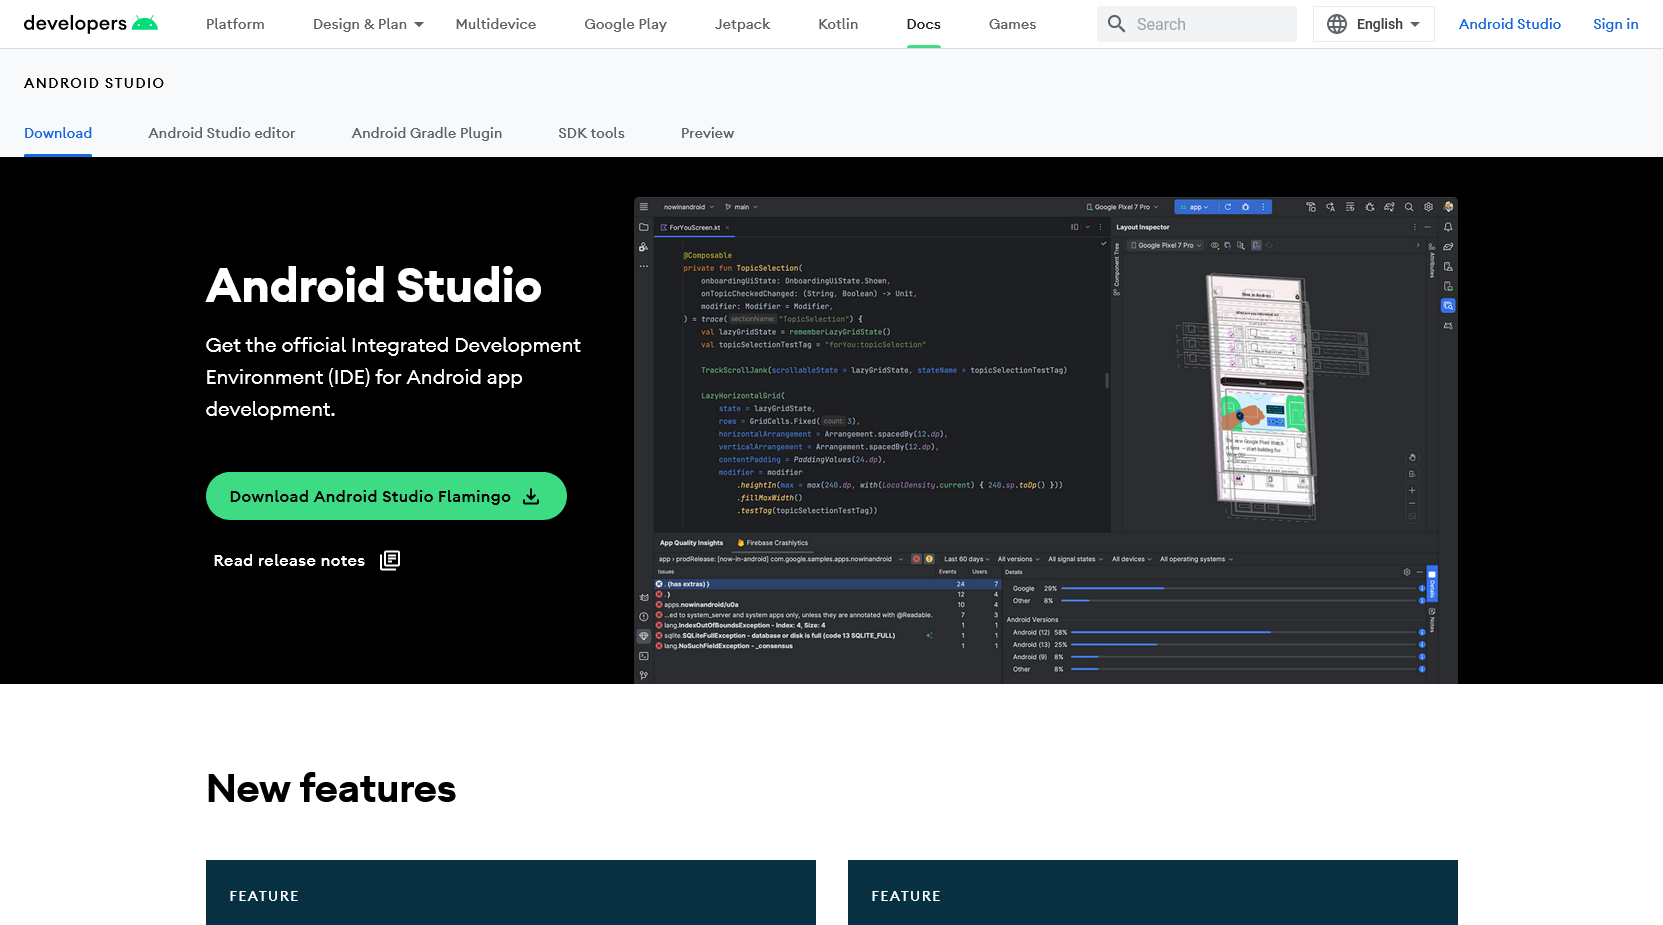
\includegraphics[width=0.99\textwidth]
        {images/android-studio/1.png}

        \caption{Скриншот}

        \label{fig:android_studio_install_1}
    \end{minipage}
    \begin{minipage}{0.49\textwidth}
        \centering

        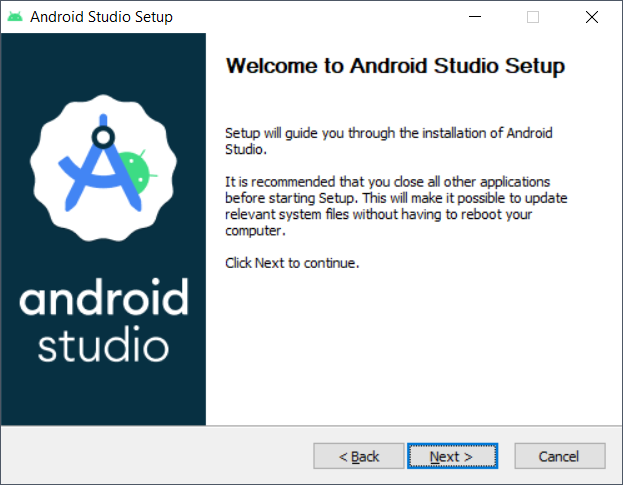
\includegraphics[width=0.99\textwidth]
        {images/android-studio/2.png}

        \caption{Скриншот}

        \label{fig:android_studio_install_2}
    \end{minipage}
\end{figure}

\begin{figure}[!phtb]
    \centering

    \begin{minipage}{0.49\textwidth}
        \centering

        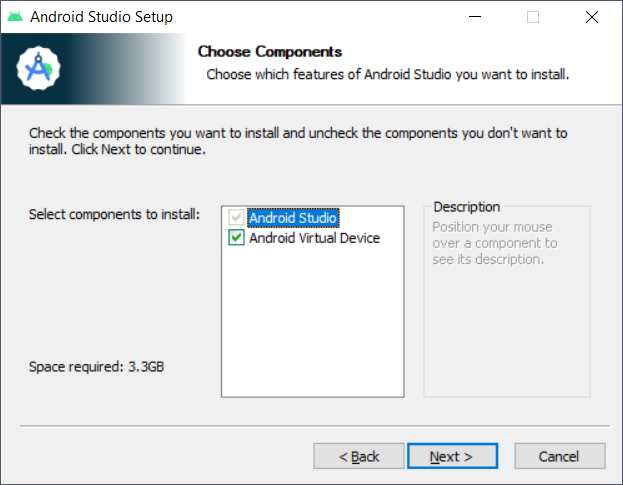
\includegraphics[width=0.99\textwidth]
        {images/android-studio/3.png}

        \caption{Скриншот}

        \label{fig:android_studio_install_3}
    \end{minipage}
    \begin{minipage}{0.49\textwidth}
        \centering

        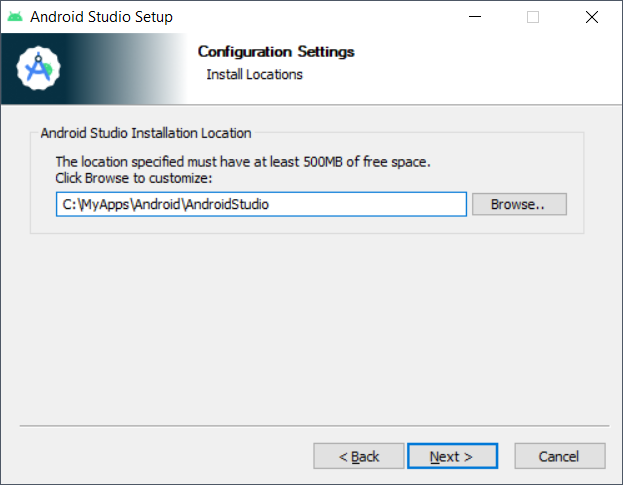
\includegraphics[width=0.99\textwidth]
        {images/android-studio/4.png}

        \caption{Скриншот}

        \label{fig:android_studio_install_4}
    \end{minipage}
\end{figure}

\begin{figure}[!phtb]
    \centering

    \begin{minipage}{0.49\textwidth}
        \centering

        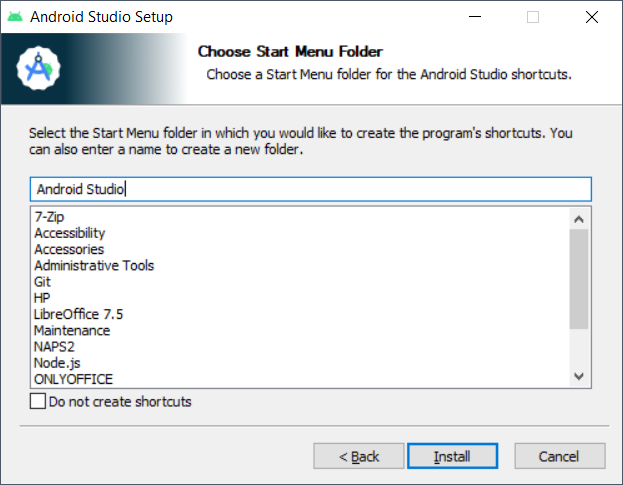
\includegraphics[width=0.99\textwidth]
        {images/android-studio/5.png}

        \caption{Скриншот}

        \label{fig:android_studio_install_5}
    \end{minipage}
    \begin{minipage}{0.49\textwidth}
        \centering

        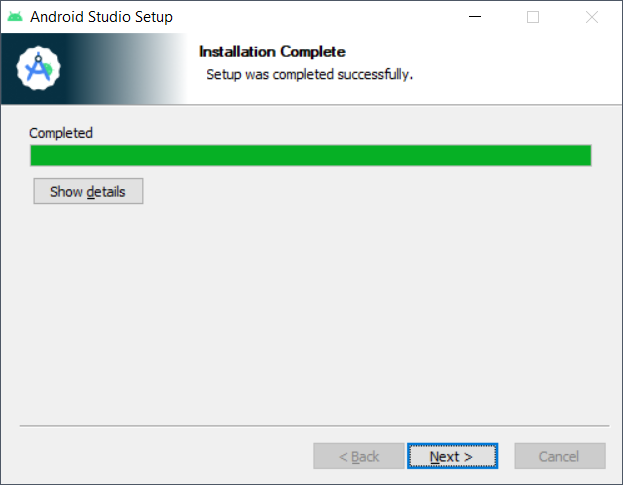
\includegraphics[width=0.99\textwidth]
        {images/android-studio/6.png}

        \caption{Скриншот}

        \label{fig:android_studio_install_6}
    \end{minipage}
\end{figure}

\begin{figure}[!phtb]
    \centering

    \begin{minipage}{0.49\textwidth}
        \centering

        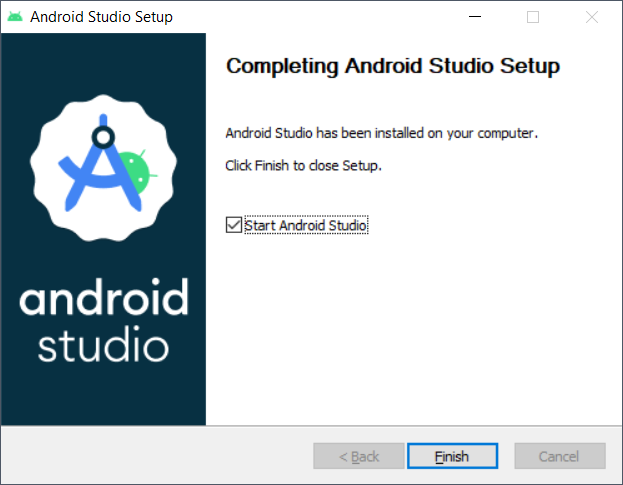
\includegraphics[width=0.99\textwidth]
        {images/android-studio/7.png}

        \caption{Скриншот}

        \label{fig:android_studio_install_7}
    \end{minipage}
    \begin{minipage}{0.49\textwidth}
        \centering

        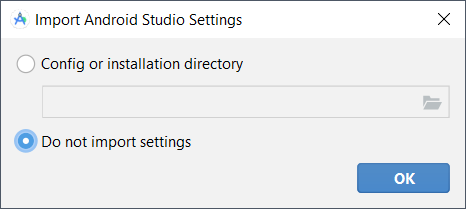
\includegraphics[width=0.99\textwidth]
        {images/android-studio/8.png}

        \caption{Скриншот}

        \label{fig:android_studio_install_8}
    \end{minipage}
\end{figure}

\begin{figure}[!phtb]
    \centering

    \begin{minipage}{0.49\textwidth}
        \centering

        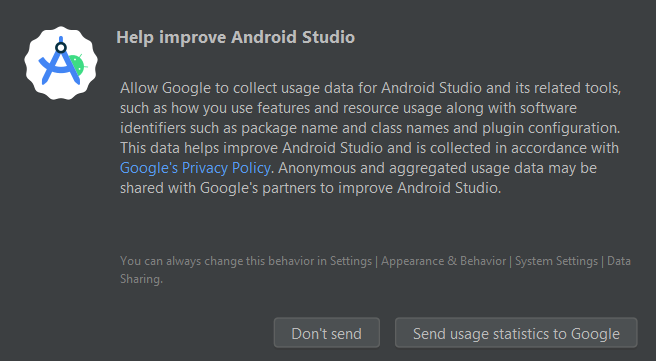
\includegraphics[width=0.99\textwidth]
        {images/android-studio/9.png}

        \caption{Скриншот}

        \label{fig:android_studio_install_9}
    \end{minipage}
    \begin{minipage}{0.49\textwidth}
        \centering

        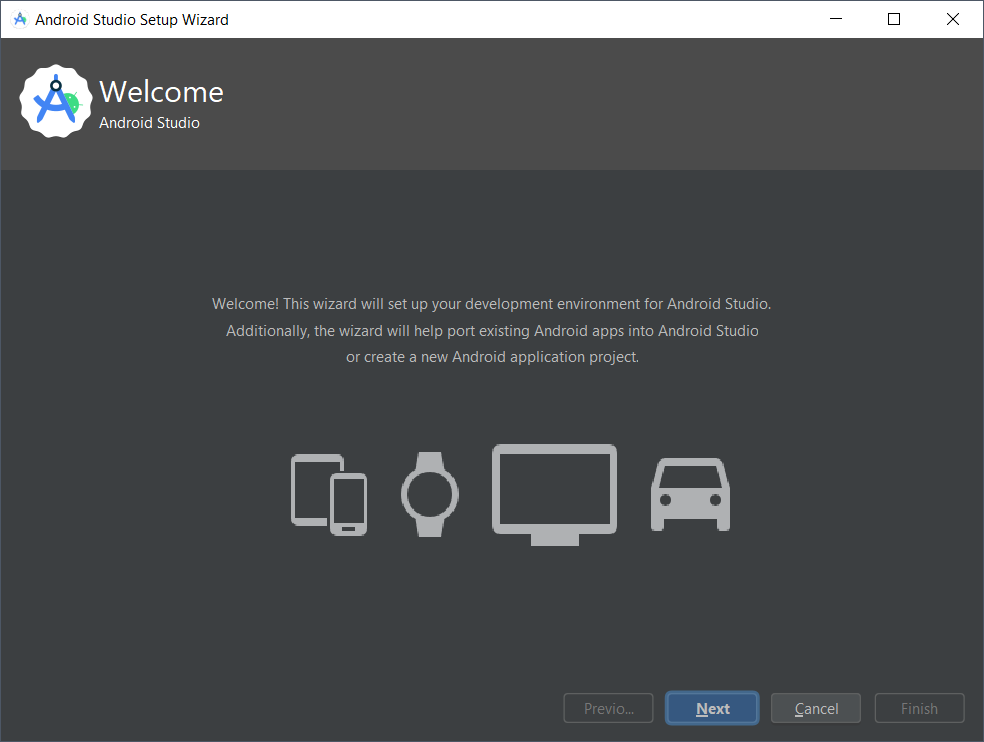
\includegraphics[width=0.99\textwidth]
        {images/android-studio/10.png}

        \caption{Скриншот}

        \label{fig:android_studio_install_10}
    \end{minipage}
\end{figure}

\begin{figure}[!phtb]
    \centering

    \begin{minipage}{0.49\textwidth}
        \centering

        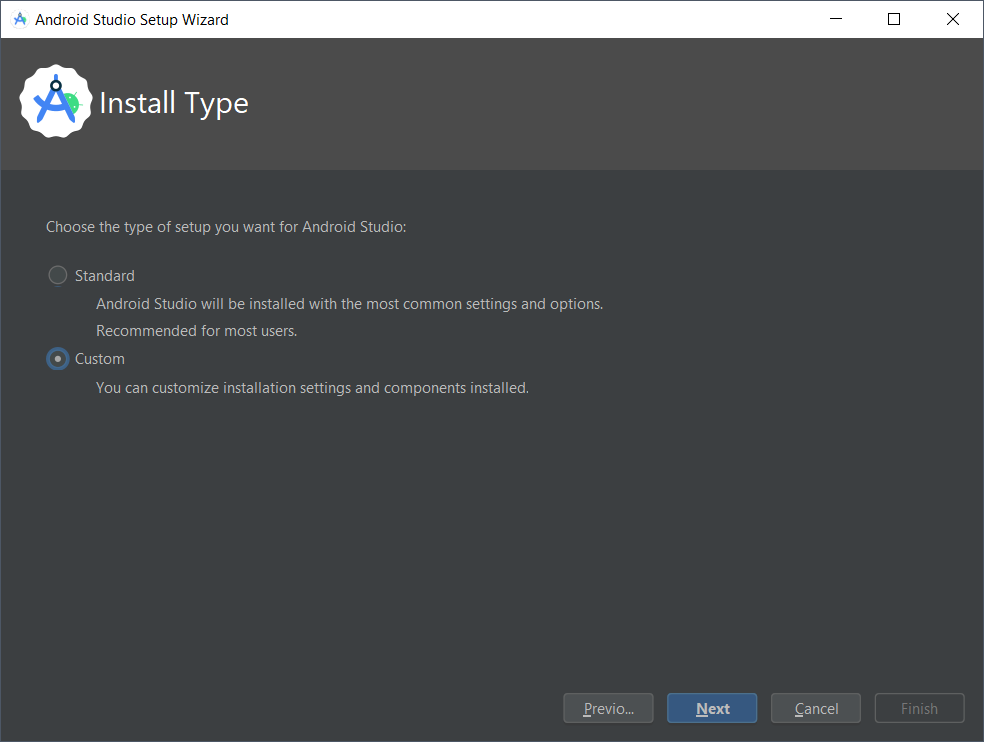
\includegraphics[width=0.99\textwidth]
        {images/android-studio/11.png}

        \caption{Скриншот}

        \label{fig:android_studio_install_11}
    \end{minipage}
    \begin{minipage}{0.49\textwidth}
        \centering

        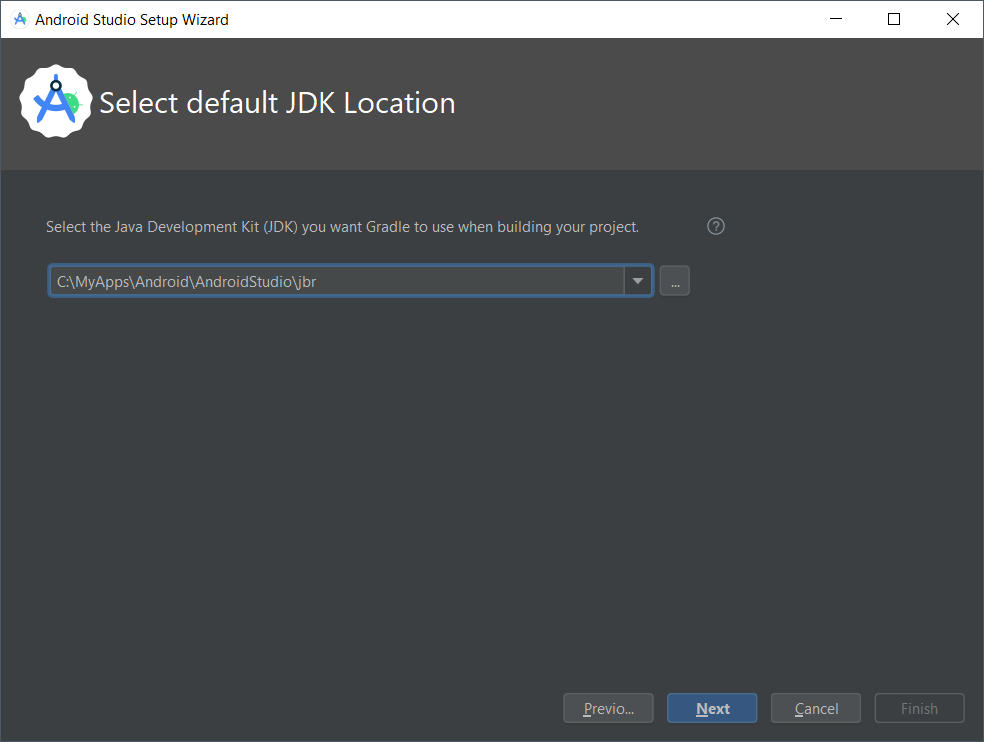
\includegraphics[width=0.99\textwidth]
        {images/android-studio/12.png}

        \caption{Скриншот}

        \label{fig:android_studio_install_12}
    \end{minipage}
\end{figure}

\begin{figure}[!phtb]
    \centering

    \begin{minipage}{0.49\textwidth}
        \centering

        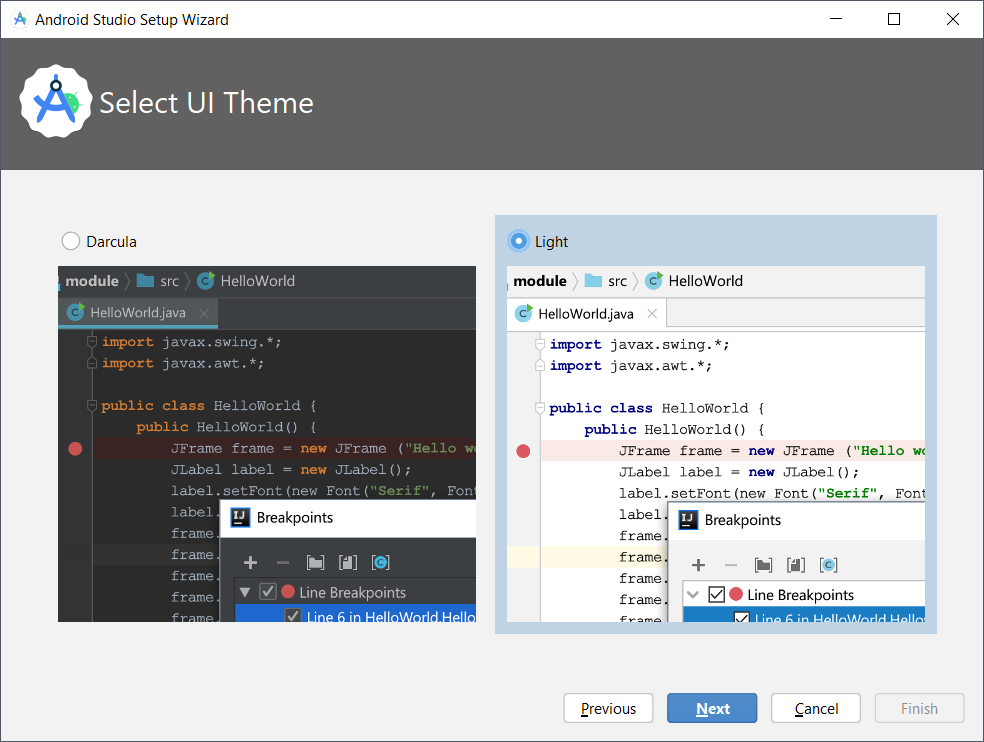
\includegraphics[width=0.99\textwidth]
        {images/android-studio/13.png}

        \caption{Скриншот}

        \label{fig:android_studio_install_13}
    \end{minipage}
    \begin{minipage}{0.49\textwidth}
        \centering

        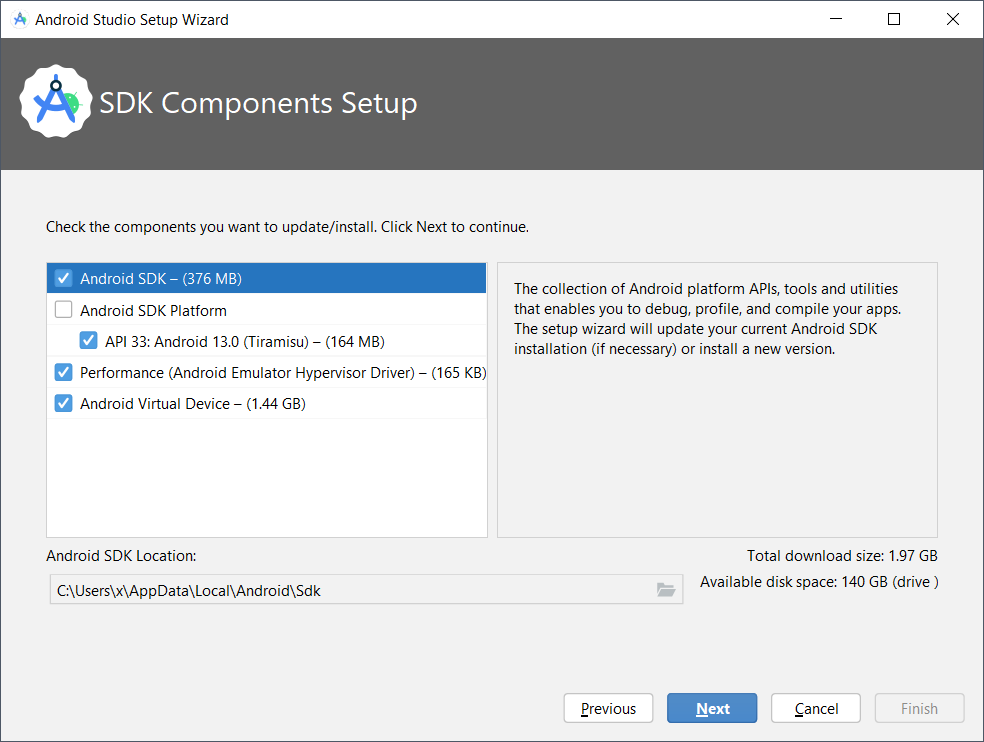
\includegraphics[width=0.99\textwidth]
        {images/android-studio/14.png}

        \caption{Скриншот}

        \label{fig:android_studio_install_14}
    \end{minipage}
\end{figure}

\begin{figure}[!phtb]
    \centering

    \begin{minipage}{0.49\textwidth}
        \centering

        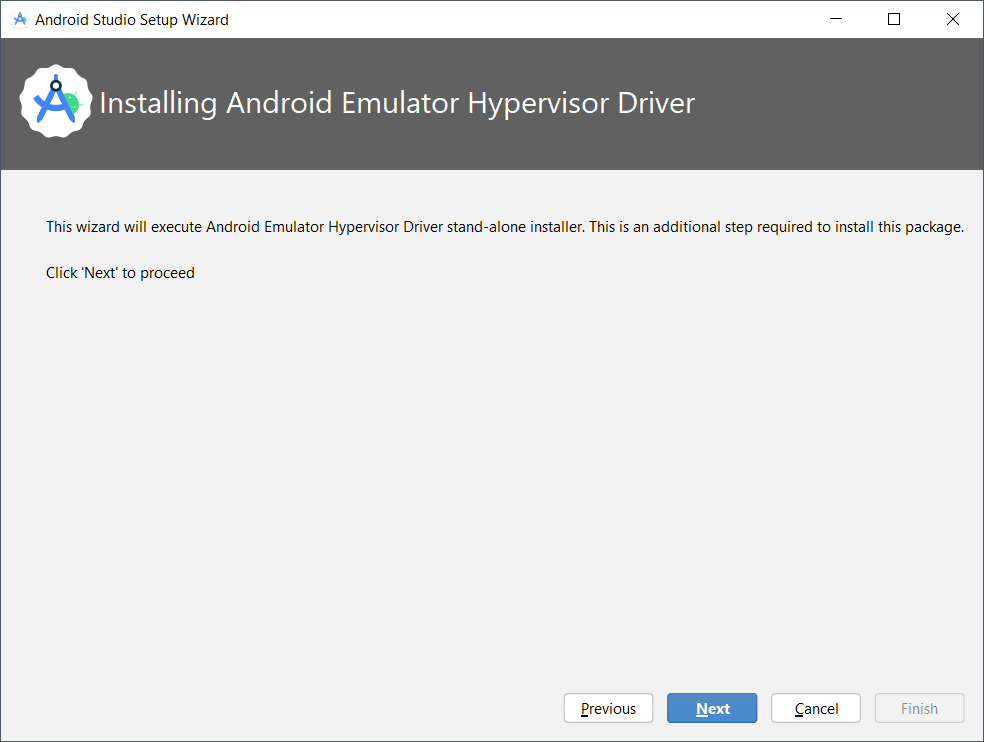
\includegraphics[width=0.99\textwidth]
        {images/android-studio/15.png}

        \caption{Скриншот}

        \label{fig:android_studio_install_15}
    \end{minipage}
    \begin{minipage}{0.49\textwidth}
        \centering

        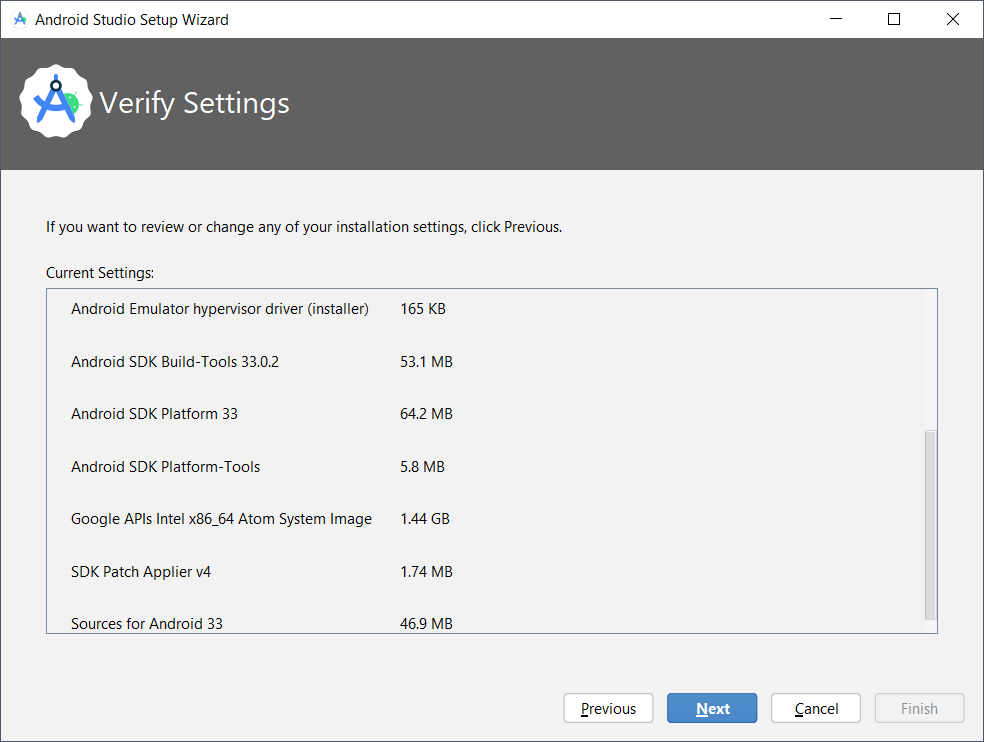
\includegraphics[width=0.99\textwidth]
        {images/android-studio/16.png}

        \caption{Скриншот}

        \label{fig:android_studio_install_16}
    \end{minipage}
\end{figure}

\begin{figure}[!phtb]
    \centering

    \begin{minipage}{0.49\textwidth}
        \centering

        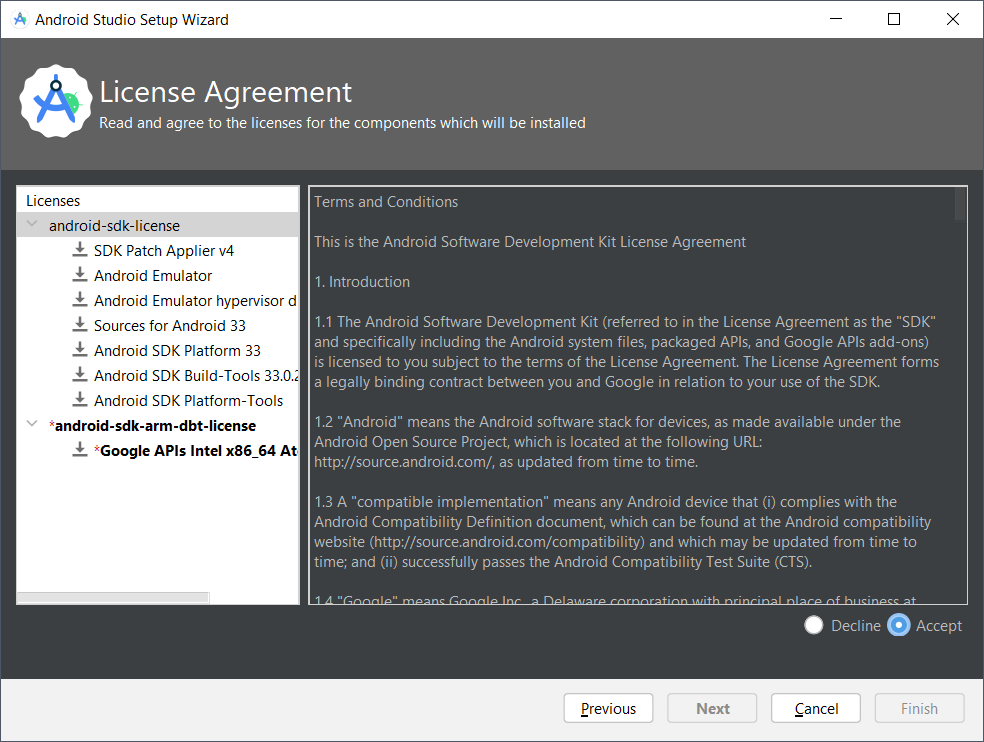
\includegraphics[width=0.99\textwidth]
        {images/android-studio/17.png}

        \caption{Скриншот}

        \label{fig:android_studio_install_17}
    \end{minipage}
    \begin{minipage}{0.49\textwidth}
        \centering

        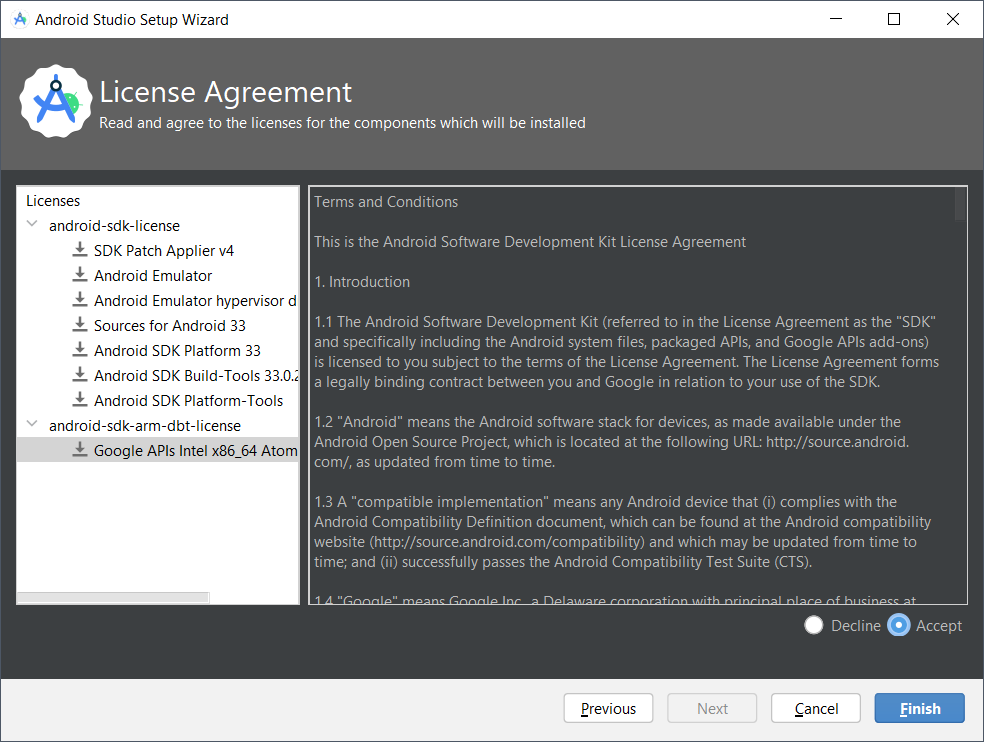
\includegraphics[width=0.99\textwidth]
        {images/android-studio/18.png}

        \caption{Скриншот}

        \label{fig:android_studio_install_18}
    \end{minipage}
\end{figure}

\begin{figure}[!phtb]
    \centering

    \begin{minipage}{0.49\textwidth}
        \centering

        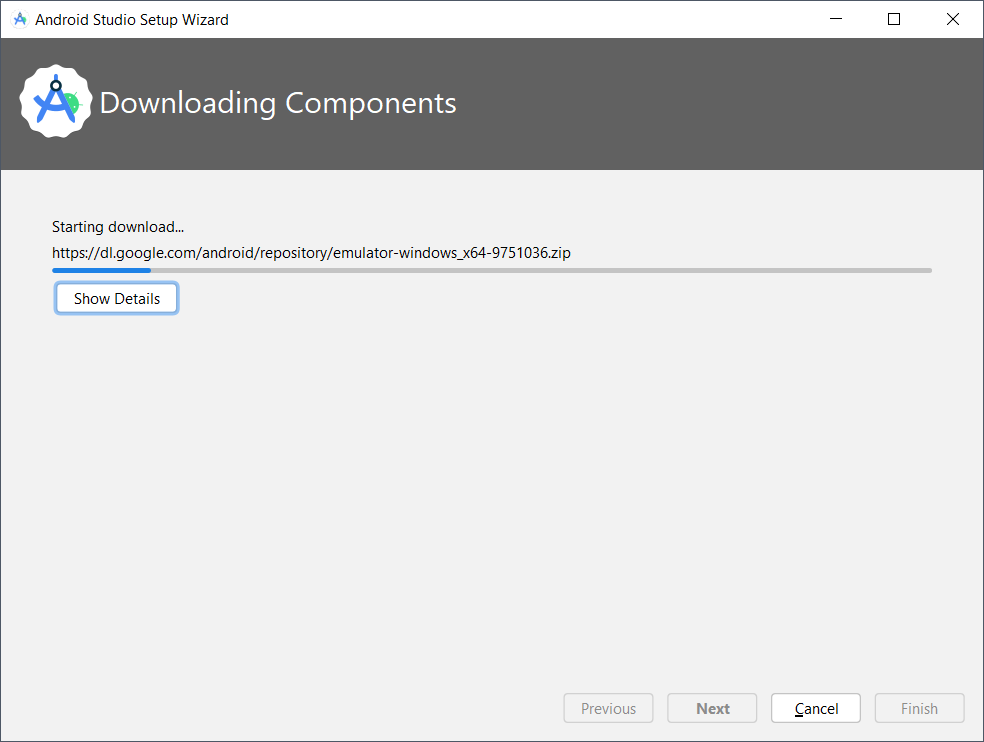
\includegraphics[width=0.99\textwidth]
        {images/android-studio/19.png}

        \caption{Скриншот}

        \label{fig:android_studio_install_19}
    \end{minipage}
    \begin{minipage}{0.49\textwidth}
        \centering

        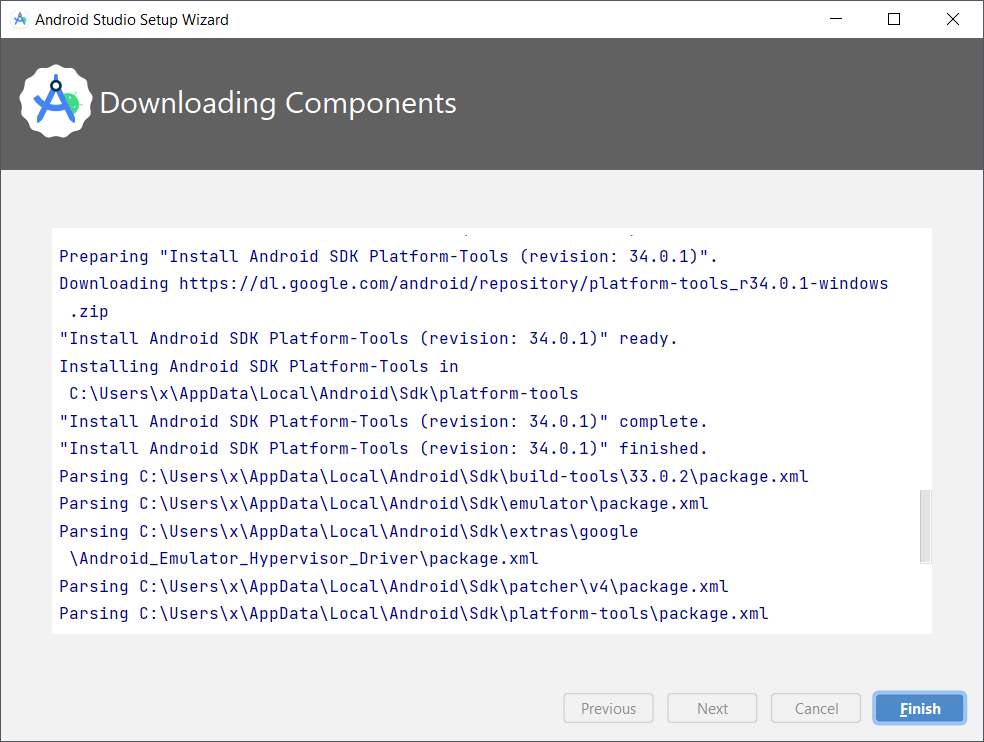
\includegraphics[width=0.99\textwidth]
        {images/android-studio/20.png}

        \caption{Скриншот}

        \label{fig:android_studio_install_20}
    \end{minipage}
\end{figure}

\subsection{Создание проекта в Android Studio}

Перед тем как разрабатывать на React Native на языке Type Script (Java Script),
нужно запустить проект на Kotlin или Java в Android Studio, для того,
чтобы применился эмулятор Android.
Если захотим сменить устройство, то прийдется также запустить пустой проект на Kotlin или Java c другим устройством.

После установки Android Studio появиться окно с предложением о создании проекта.

Если окно не появилось, то запустите Android Studio.

\begin{itemize}
    \item жмём <<New Project>> (см. рисунок~\ref{fig:android_studio_create_1});
    \item жмём <<Empty Activity>> (см. рисунок~\ref{fig:android_studio_create_2});
    \item жмём <<Next>> (см. рисунок~\ref{fig:android_studio_create_3});
    \item если появится сообщение о блокировке, то разрешает доступ (см. рисунок~\ref{fig:android_studio_create_4});
    \item ждём пока справа снизу пропадет полоса загрузки (см. рисунок~\ref{fig:android_studio_create_5});
    \item жмём зеленый треугольник справа сверху (см. рисунок~\ref{fig:android_studio_create_6});
    \item если появился эмулятор Android с запущеным приложением, то можно закрывать приложение,
    по красному квадрату справа сверху (см. рисунок~\ref{fig:android_studio_create_7});
    \item закрываем Android Studio на крестик.
\end{itemize}

\begin{figure}[!phtb]
    \centering

    \begin{minipage}{0.49\textwidth}
        \centering

        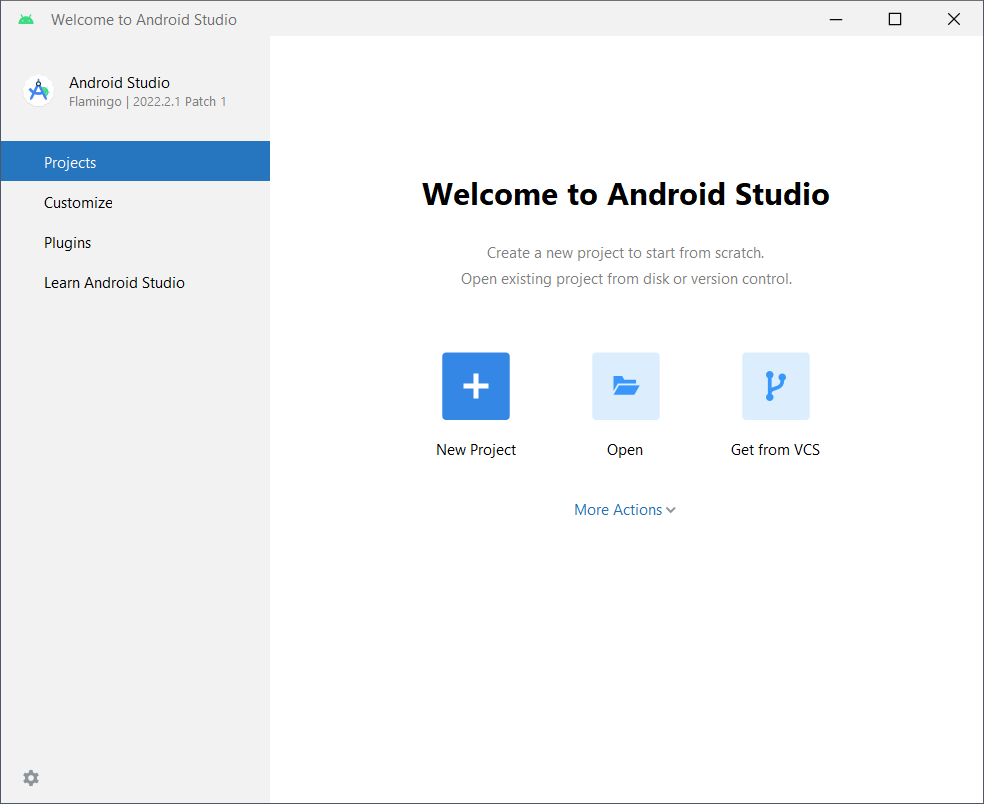
\includegraphics[width=0.99\textwidth]
        {images/android-studio-create/1.png}

        \caption{Скриншот}

        \label{fig:android_studio_create_1}
    \end{minipage}
    \begin{minipage}{0.49\textwidth}
        \centering

        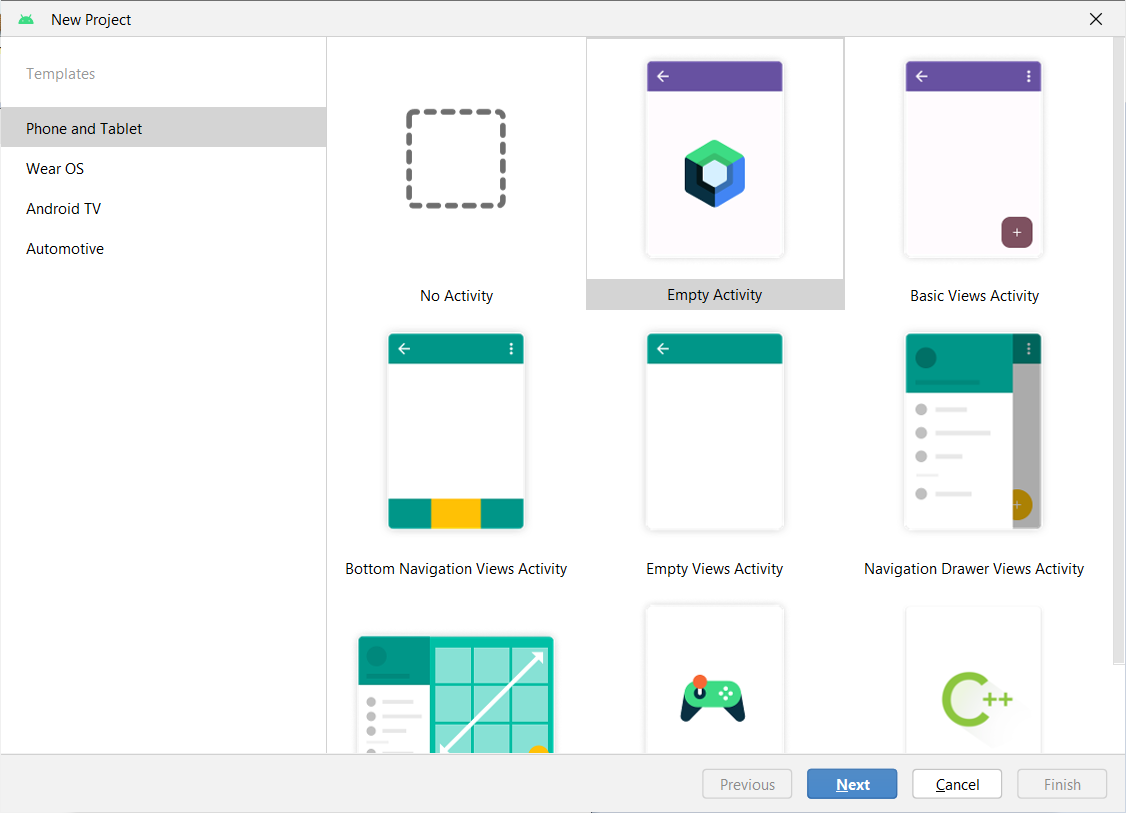
\includegraphics[width=0.99\textwidth]
        {images/android-studio-create/2.png}

        \caption{Скриншот}

        \label{fig:android_studio_create_2}
    \end{minipage}
\end{figure}

\begin{figure}[!phtb]
    \centering

    \begin{minipage}{0.49\textwidth}
        \centering

        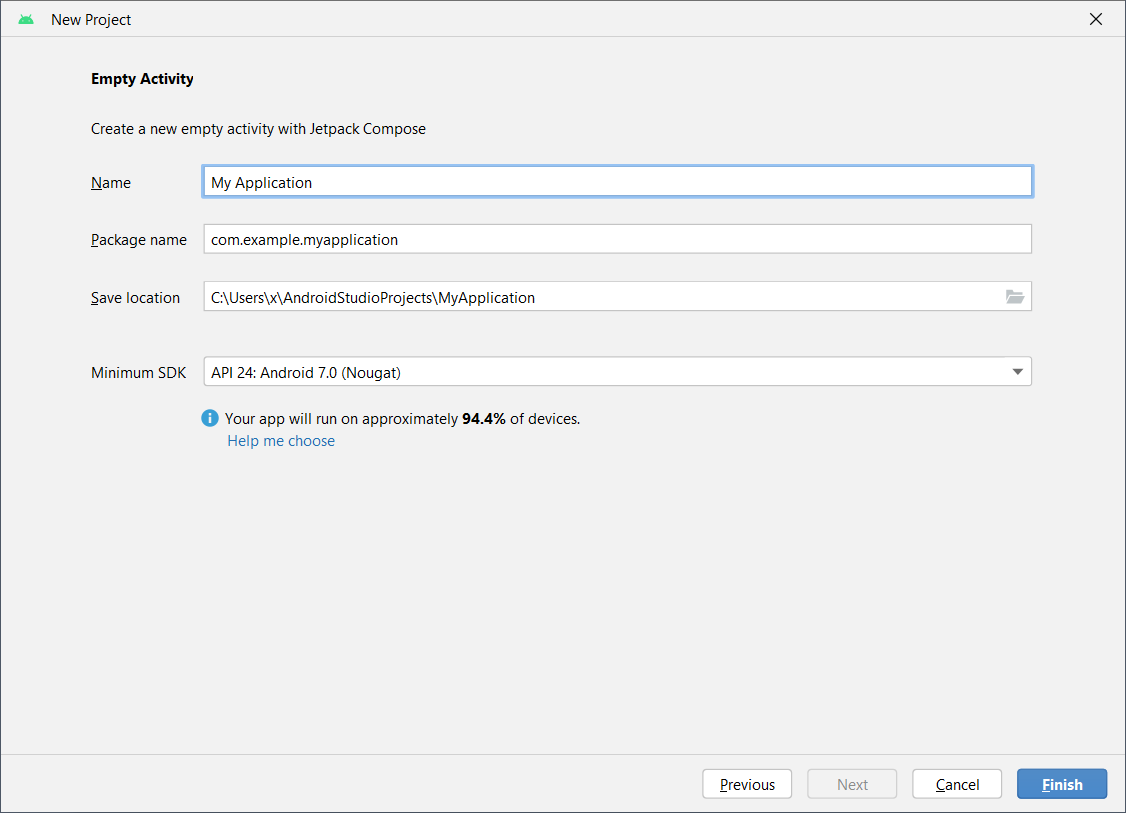
\includegraphics[width=0.99\textwidth]
        {images/android-studio-create/3.png}

        \caption{Скриншот}

        \label{fig:android_studio_create_3}
    \end{minipage}
    \begin{minipage}{0.49\textwidth}
        \centering

        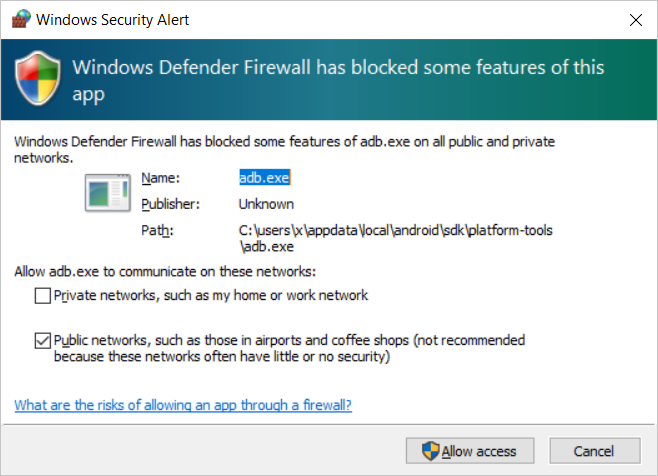
\includegraphics[width=0.99\textwidth]
        {images/android-studio-create/4.png}

        \caption{Скриншот}

        \label{fig:android_studio_create_4}
    \end{minipage}
\end{figure}

\begin{figure}[!phtb]
    \centering

    \begin{minipage}{0.49\textwidth}
        \centering

        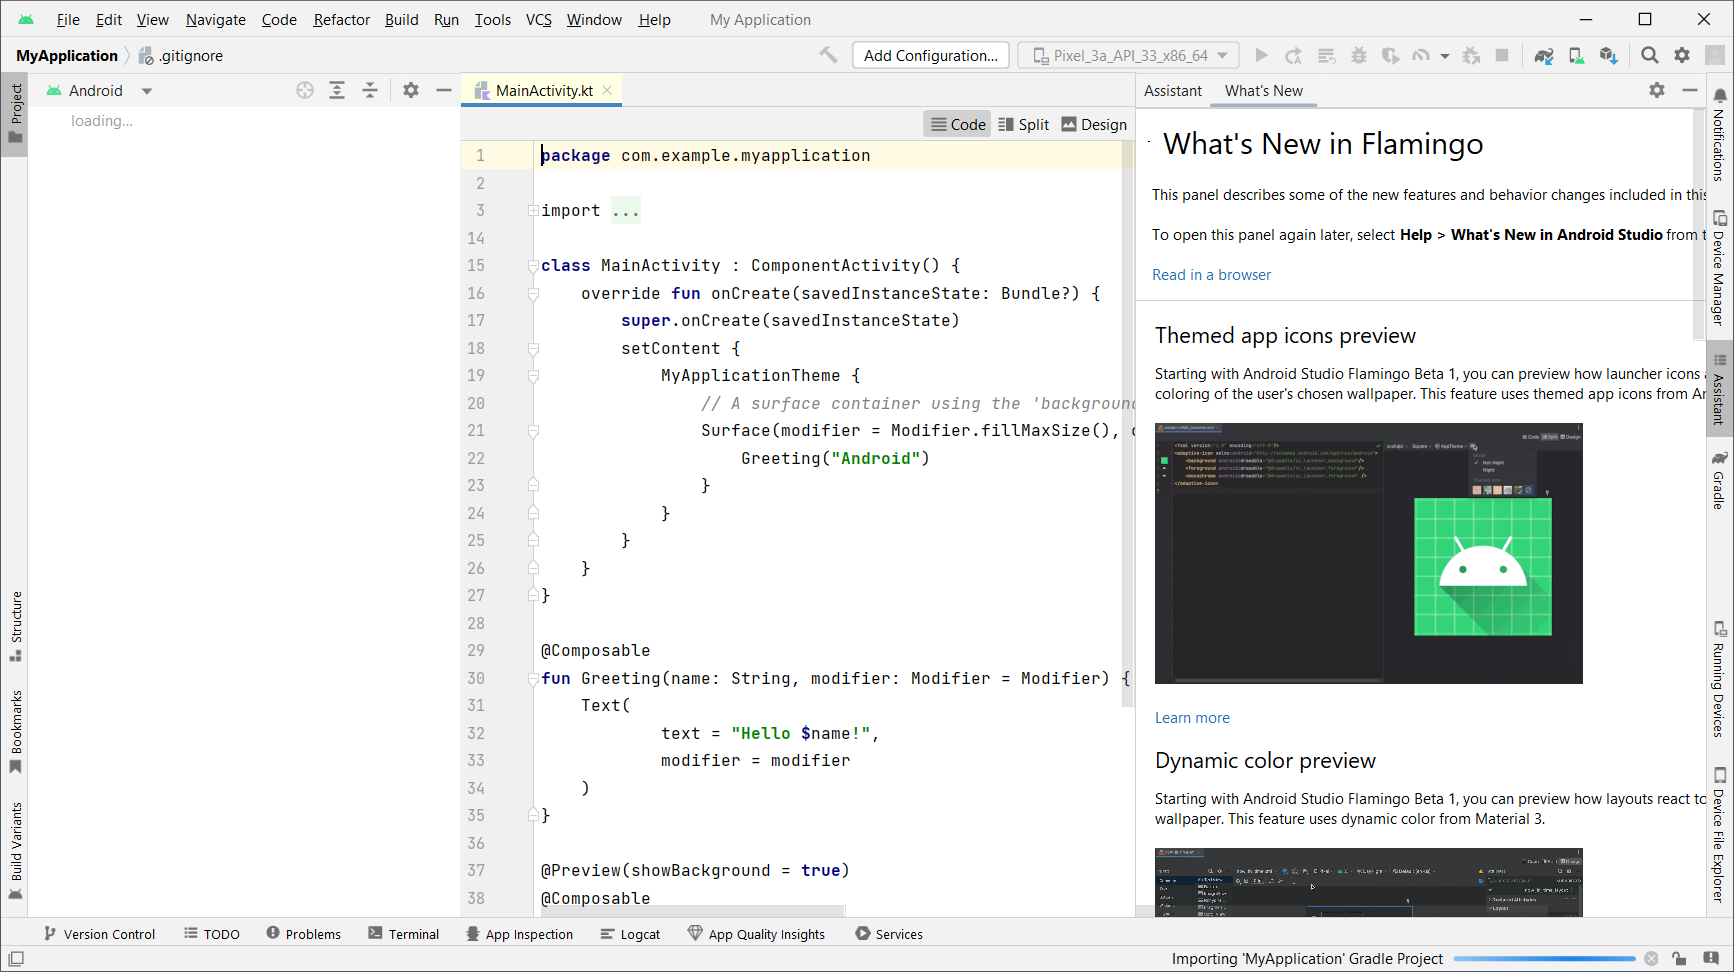
\includegraphics[width=0.99\textwidth]
        {images/android-studio-create/5.png}

        \caption{Скриншот}

        \label{fig:android_studio_create_5}
    \end{minipage}
    \begin{minipage}{0.49\textwidth}
        \centering

        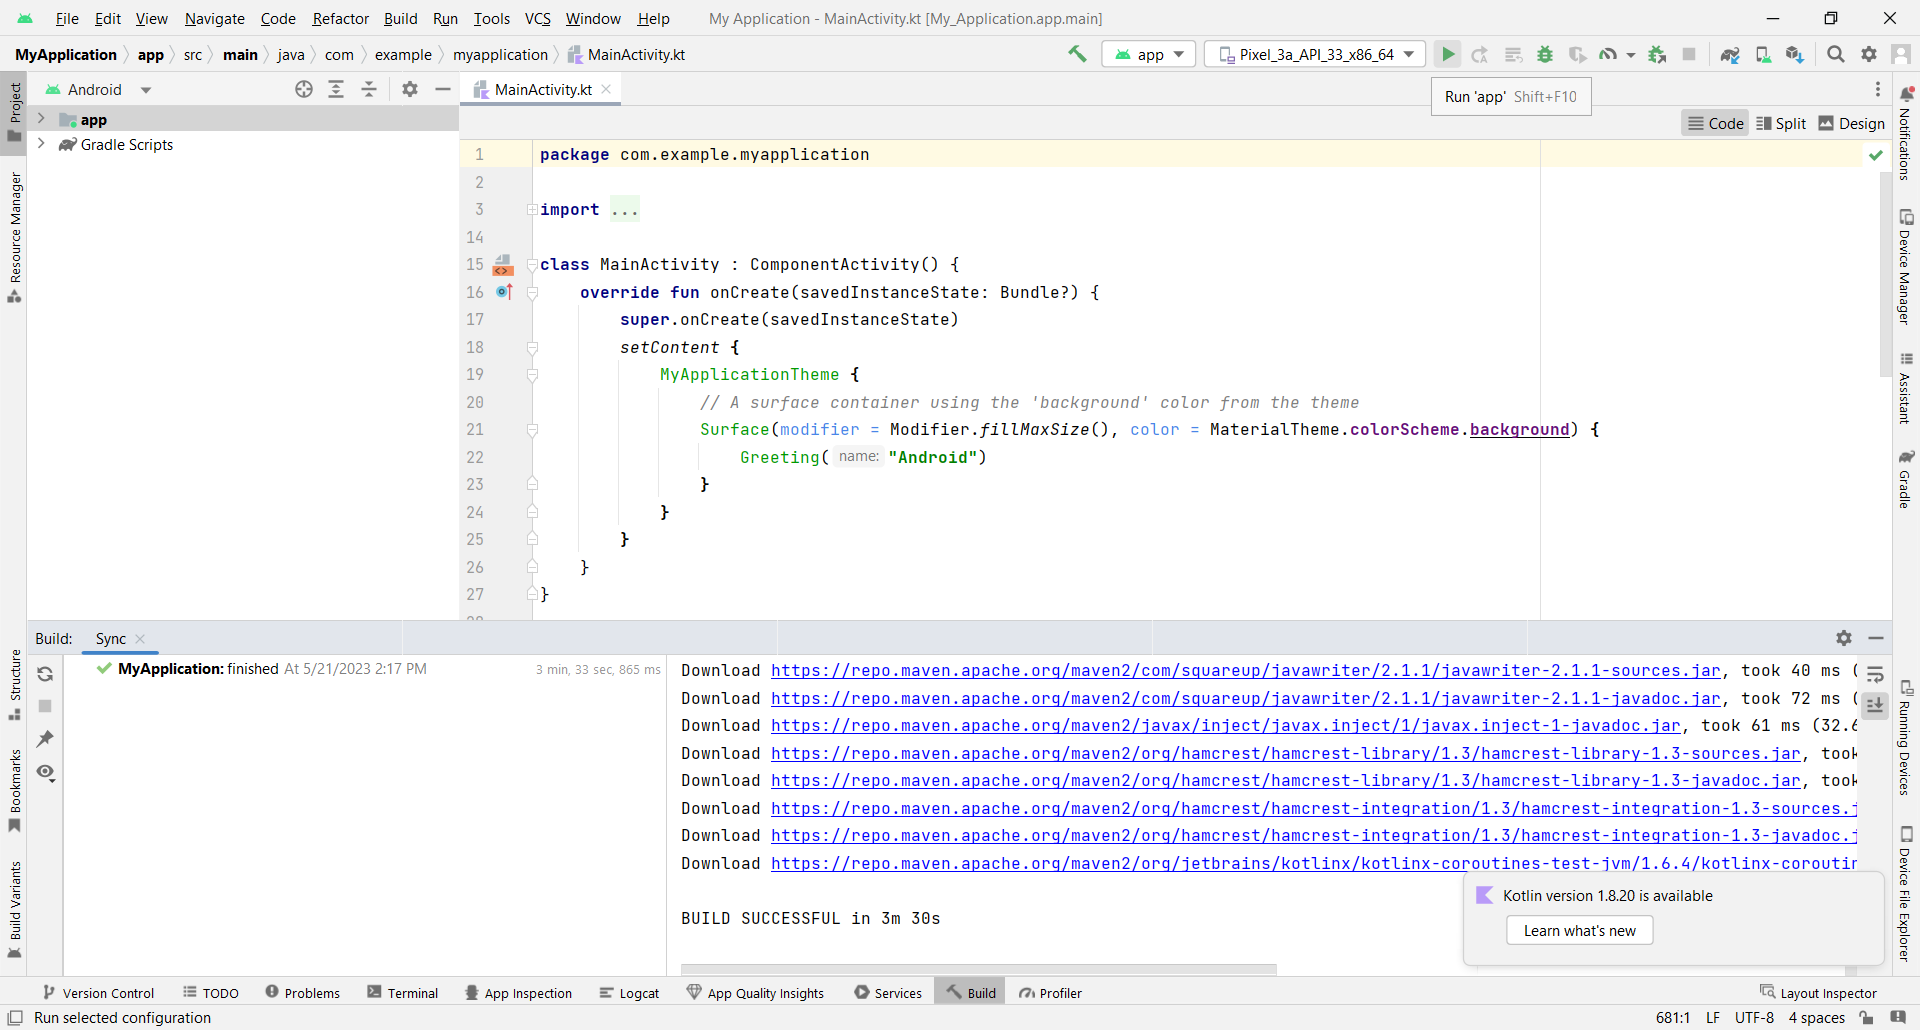
\includegraphics[width=0.99\textwidth]
        {images/android-studio-create/6.png}

        \caption{Скриншот}

        \label{fig:android_studio_create_6}
    \end{minipage}
\end{figure}

\begin{figure}[!phtb]

    \centering

    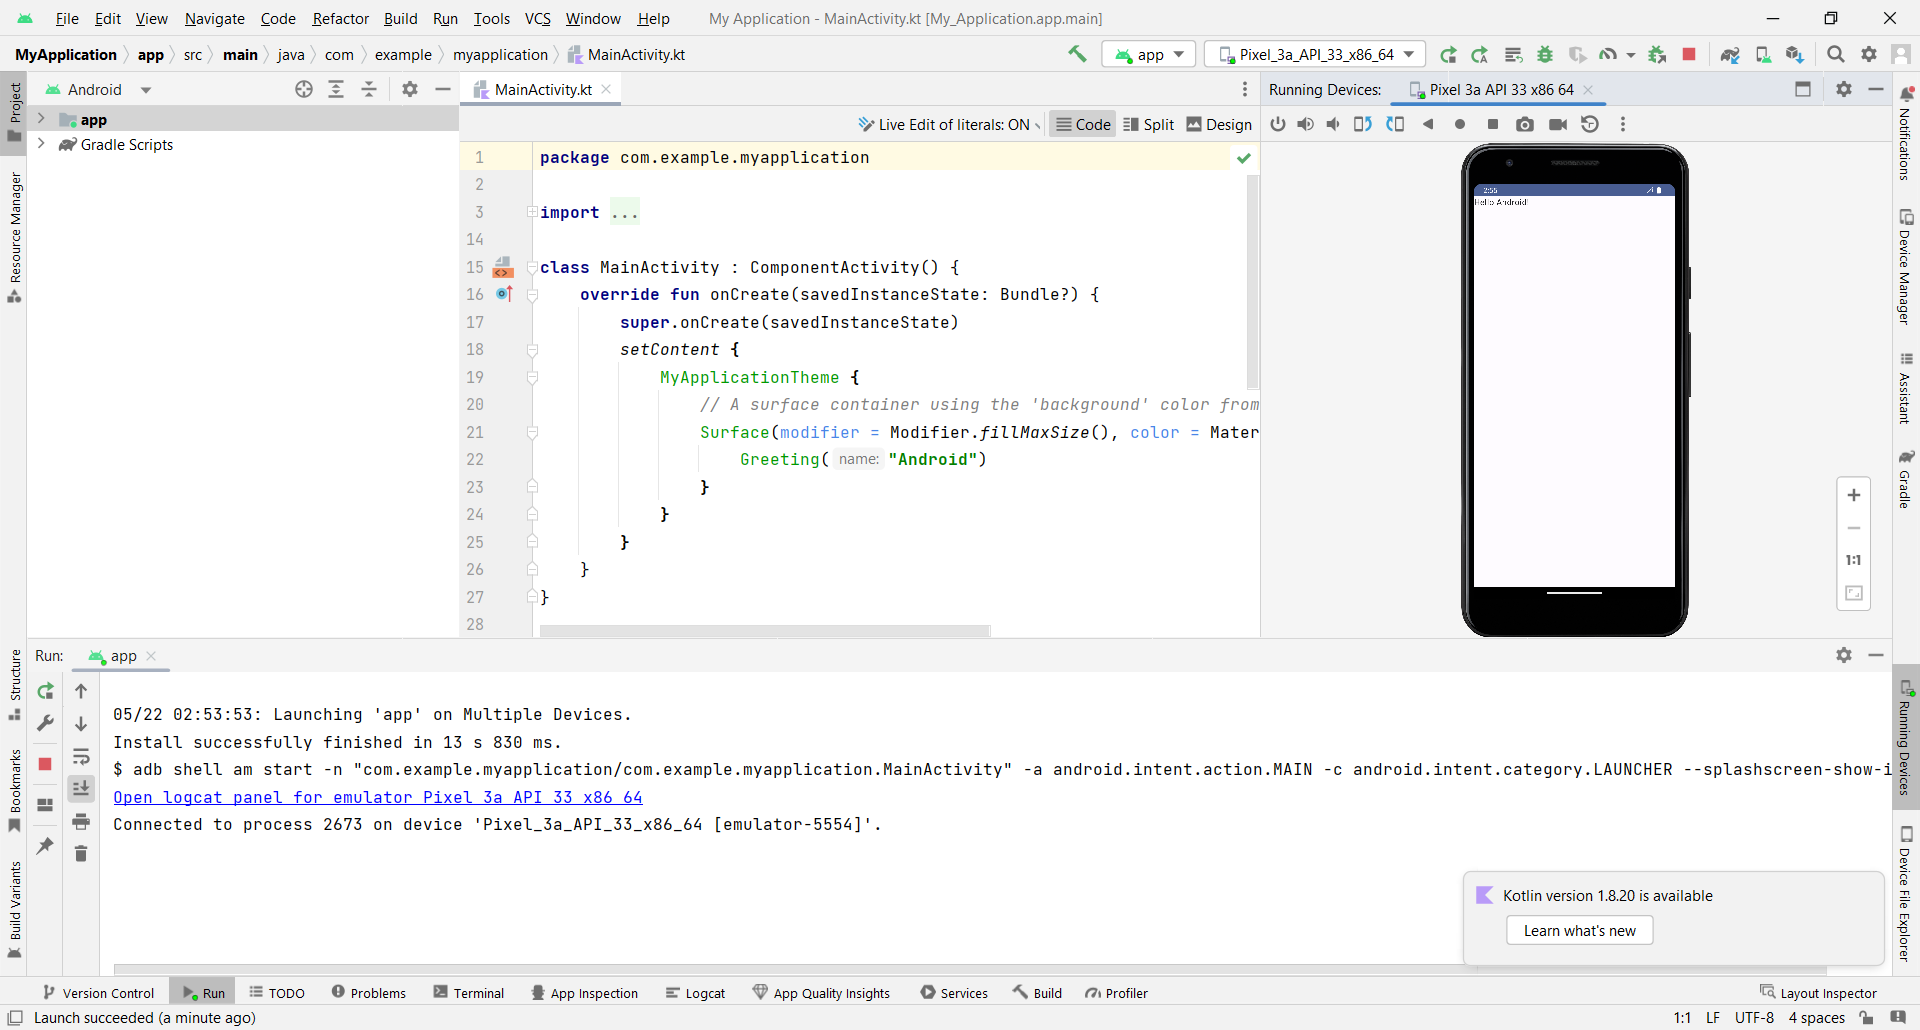
\includegraphics[width=0.50\textwidth]
    {images/android-studio-create/7.png}

    \caption{Скриншот}

    \label{fig:android_studio_create_7}

\end{figure}

\subsection{Открытие переменных окружения в Windows 10} \label{sect:Win10env}

Алгоритм открытия окна переменных окружения в Win10:

\begin{itemize}
    \item[-] открываем окно выполнить нажатием клавиш <<Win>> + <<R>>;
    \item[-] пишем <<control>> и жмём <<Enter>>;
    \item[-] в открытой панели управления выбираем <<System and Security>>;
    \item[-] выбираем <<System>>;
    \item[-] выбираем <<Advanced system settings>>;
    \item[-] жмём кнопку <<Environment Variables>>;
\end{itemize}

\subsection{Добавляем переменную окружения ANDROID\_HOME}

Откроейте окно с переменными окружения (см. главу~\ref{sect:Win10env}).

Алгоритм добавления переменной <<ANDROID\_HOME>>:
\begin{itemize}
    \item[-] жмём кнопку <<New...>>;
    \item[-] вводим <<ANDROID\_HOME>> в поле <<Variable name>>;
    \item[-] вводим <<\%LOCALAPPDATA\%{\char`\\}Android{\char`\\}Sdk>> в поле <<Variable value>>;
    \item[-] жмём кнопку <<OK>>.
\end{itemize}

\subsection{Добавляем переменную окружения путь Android SKD}

Откроейте окно с переменными окружения (см. главу~\ref{sect:Win10env}).

Добавляем путь в PATH:
\begin{itemize}
    \item[-] выбираем переменную <<PATH>>;
    \item[-] жмём кнопку <<Edit...>>;
    \item[-] жмём кнопку <<New>>;
    \item[-] вводим <<\%LOCALAPPDATA\%{\char`\\}Android{\char`\\}Sdk{\char`\\}platform-tools>>;
    \item[-] жмём кнопку <<OK>>.
\end{itemize}

\subsection{Добавляем переменную окружения JAVA\_HOME}

Откроейте окно с переменными окружения (см. главу~\ref{sect:Win10env}).

Скопируйте себе в папку <<C:{\char`\\}{\char`\\}MyApps{\char`\\}OpenJds>> содержимое, которое находится
на диске приложеном в дипломному проекту в папке Downloads.

Добавляем переменную <<JAVA\_HOME>>:
\begin{itemize}
    \item[-] жмём <<New...>>;
    \item[-] вводим <<JAVA\_HOME>> в поле <<Variable name>> ;
    \item[-] вводим <<C:{\char`\\}{\char`\\}MyApps{\char`\\}OpenJds{\char`\\}openjdk-20.0.1\_windows-x64\_bin{\char`\\}\\jdk-20.0.1>>
    в поле <<Variable value>>;
    \item[-] жмём кнопку <<OK>>.
\end{itemize}

\subsection{Запуск мобильного приложения для разработки}

Перед разработкой мобильного приложения должна быть установлена\\ NodeJS (см. главу~\ref{sect:nodejs}).

Мобильное приложение нет смысла разрабатывать без запущеной серверной части (см. главу~\ref{sect:backend}).

Алгоритм запуска мобильного приложения для разработки:
\begin{enumerate}
    \item[-] открываем папку <<dp\_mobile>>;
    \item[-] открываем консоль;
    \item[-] переходим папку sources командой: <<cd sources>>.
    \item[-] если не установлены пакеты npm, то есть нет папки node\_modules, то устанавливаем командой <<yarn>>;
    \item[-] запускаем командой <<yarn start>>;
    \item[-] когда появится меню, то жмём <<a>>, чтобы открыть эмулятор Android.
\end{enumerate}
